\documentclass[a4paper,12pt,twoside]{book}
\usepackage{mei/mei}

% Diagrams exported from docs/diagrams are included as PDF.
% On Overleaf you can upload the .svg directly and it is converted on compile;
% locally, export each images/*.svg to images/*.pdf before building.

\title{ Secure Development and Testing Tool for Model Context Protocol
Implementations}
\author{Mário João de Araújo Pinto}
% \propostaDissertacao % ou \propostaProjeto
\propostaProjeto
\MEI
\date{\today}


\pagenumbering{roman}
%% Caso tenham mais que um orientador, colocar
%% \orientador{Nome professor \AND Nome professor}
\orientador{Prof. Nuno Lopes \AND Prof. Rui Fernandes}

% comentar se não for para usar glossários
\makeglossaries


\begin{document}

%\frontmatter
\maketitle

\begin{resumo}
A crescente adoção do Model Context Protocol (MCP) tem permitido que sistemas baseados em modelos de linguagem interajam com ferramentas externas, bases de dados e serviços, expandindo significativamente as suas capacidades. Contudo, esta maior conectividade introduz novas superfícies de ataque e riscos de segurança, incluindo ataques de prompt injection, acesso não autorizado a dados, uso indevido de ferramentas e vulnerabilidades agente-para-agente (A2A).

Esta dissertação apresenta o desenvolvimento de uma ferramenta de segurança para implementações MCP, com foco na identificação, mitigação e prevenção de vulnerabilidades específicas deste ecossistema. Seguindo uma abordagem de Design Science Research, foi concebido e validado um artefacto técnico aplicável a contextos reais.

O principal contributo consiste numa ferramenta que combina duas análises complementares sobre a mesma taxonomia de vulnerabilidades: uma análise dinâmica que se liga a um servidor MCP em execução, classifica as suas ferramentas com recurso a um Large Language Model e executa ataques adversariais controlados, e uma análise estática que inspeciona o código-fonte de um servidor sem o executar. O objetivo é estabelecer boas práticas de segurança que reduzam o risco associado à adoção do MCP em ambientes empresariais e infraestruturas críticas.

\vspace{1em}
\noindent\textbf{Palavras-chave:} Model Context Protocol (MCP); Segurança de Sistemas de IA; \textit{Prompt Injection}; Testes Adversariais; Análise Estática e Dinâmica; \textit{Large Language Models}; \textit{Design Science Research}


\end{resumo}

\begin{abstract}
The increasing adoption of the Model Context Protocol (MCP) has enabled language model--based systems to interact with external tools, databases, and services, significantly expanding their capabilities. However, this increased connectivity introduces new attack surfaces and security risks, including prompt injection attacks, unauthorized data access, tool misuse, and agent-to-agent (A2A) vulnerabilities.

This dissertation presents the development of a security tool for MCP implementations, focusing on the identification, mitigation, and prevention of vulnerabilities specific to this ecosystem. Following a Design Science Research approach, a technical artifact was designed and validated for real-world application.

The main contribution is a tool that combines two complementary analyses over a single vulnerability taxonomy: a dynamic analysis that connects to a running MCP server, classifies its exposed tools with a Large Language Model, and executes controlled adversarial attacks, and a static analysis that inspects a server's source code without executing it. The goal is to establish security best practices that reduce the risks associated with MCP adoption in enterprise and critical infrastructure environments.


\vspace{1em}
\noindent\textbf{Keywords:} Model Context Protocol (MCP); AI Systems Security; Prompt Injection; Adversarial Testing; Static and Dynamic Analysis; Large Language Models; Design Science Research
\end{abstract}

%% Comment the following part if you are not acknowledging anybody
%\begin{agradecimentos}
%A secção de agradecimentos é a parte pessoal do documento, e o único sítio onde o aluno pode escrever de forma menos formal, usando o tipo de linguagem que lhe parecer adequado para as pessoas a quem agradece.
%\end{agradecimentos}


\tableofcontents

% comentar se nao tiver figuras
\listoffigures

% comentar se nao tiver tabelas
%\listoftables

% comentar se nao se quiser lista de listagens
%\lstlistoflistings

% Commentar proximas duas linhas se nao for para usar acronimos



 
 \newacronym{http}{HTTP}{HyperText Transfer Protocol}

\newacronym{ai}{AI}{Artificial Intelligence}
\newacronym{llm}{LLM}{Large Language Model}
\newacronym{mcp}{MCP}{Model Context Protocol}
\newacronym{a2a}{A2A}{Agent-to-Agent}
\newacronym{api}{API}{Application Programming Interface}
\newacronym{cicd}{CI/CD}{Continuous Integration and Continuous Deployment}
\newacronym{dsr}{DSR}{Design Science Research}
\newacronym{ssdf}{SSDF}{Secure Software Development Framework}
\newacronym{nist}{NIST}{National Institute of Standards and Technology}
\newacronym{airmf}{AI RMF}{Artificial Intelligence Risk Management Framework}
\newacronym{ml}{ML}{Machine Learning}


\newacronym{stride}{STRIDE}{Spoofing, Tampering, Repudiation, Information Disclosure, Denial of Service, Elevation of Privilege}
\newacronym{ssrf}{SSRF}{Server-Side Request Forgery}
\newacronym{dos}{DoS}{Denial of Service}
\newacronym{oauth}{OAuth}{Open Authorization}
\newacronym{pkce}{PKCE}{Proof Key for Code Exchange}
\newacronym{sdk}{SDK}{Software Development Kit}
\newacronym{orm}{ORM}{Object-Relational Mapping}
\newacronym{rest}{REST}{Representational State Transfer}
\newacronym{ast}{AST}{Abstract Syntax Tree}
\newacronym{dast}{DAST}{Dynamic Application Security Testing}
\newacronym{sast}{SAST}{Static Application Security Testing}

% "OWASP Top 10 for LLM Applications" (chap3, taxonomy section)
\newacronym{owasp}{OWASP}{Open Worldwide Application Security Project}

% "MITRE ATLAS mappings" (chap3, taxonomy section)
\newacronym{atlas}{ATLAS}{Adversarial Threat Landscape for Artificial-Intelligence Systems}

% "SQL Injection" (taxonomy table)
\newacronym{sql}{SQL}{Structured Query Language}

% "JSON columns" / "parsed as JSON" (data model, deserialization row)
\newacronym{json}{JSON}{JavaScript Object Notation}

% "JSON, YAML, or pickled data" (deserialization row)
\newacronym{yaml}{YAML}{YAML Ain't Markup Language}

% "URL or host parameters" / "The URL, headers" (SSRF row, persistence)
\newacronym{url}{URL}{Uniform Resource Locator}


% -> acronimos.tex
\newacronym{https}{HTTPS}{HyperText Transfer Protocol Secure}
\newacronym{jsonrpc}{JSON-RPC}{JSON Remote Procedure Call}
\newacronym{cvss}{CVSS}{Common Vulnerability Scoring System}
\newacronym{cia}{CIA}{Confidentiality, Integrity, Availability}
\newacronym{rag}{RAG}{Retrieval-Augmented Generation}

\printglossary[type=\acronymtype,title={Acronyms \& Abbreviations}]

% Commentar proximas duas linhas se nao for para usar glossarios
\newglossaryentry{prompt_injection}{
    name=Prompt Injection,
    description={Attack technique in which malicious instructions are embedded within input prompts to manipulate the behavior of a language model and override system-level constraints}
}

\newglossaryentry{static_analysis}{
    name=Static Analysis,
    description={Security testing technique that examines source code without executing it in order to identify structural vulnerabilities and insecure patterns}
}

\newglossaryentry{dynamic_testing}{
    name=Dynamic Testing,
    description={Security testing approach that evaluates a system during runtime to identify vulnerabilities under real execution conditions}
}

\newglossaryentry{threat_modeling}{
    name=Threat Modeling,
    description={Structured methodology for identifying, analyzing, and categorizing potential security threats across system components and trust boundaries}
}

\newglossaryentry{defense_in_depth}{
    name=Defense-in-Depth,
    description={Security strategy based on layering multiple defensive mechanisms to reduce the risk of system compromise}
}

\newglossaryentry{zero_trust}{
    name=Zero Trust,
    description={Security model based on the principle of never trusting and always verifying, requiring strict identity validation and access control regardless of network location}
}

\newglossaryentry{intrusion_detection}{
    name=Intrusion Detection,
    description={Process of monitoring systems and networks to identify malicious activities or policy violations}
}


\newglossaryentry{human_in_the_loop}{
    name=Human-in-the-Loop,
    description={Control pattern that requires an explicit human approval before an automated process proceeds to an action with real effects, used here as the gate between read-only discovery and live attack traffic}
}

\newglossaryentry{payload}{
    name=Payload,
    description={Crafted input embedded in a tool call with the intent of reaching a vulnerable code path and triggering or revealing a security weakness}
}

\newglossaryentry{sink}{
    name=Sink,
    description={Point in a program where externally controlled input reaches a sensitive operation, such as a shell command, database query, or file-system access}
}

\newglossaryentry{canary_string}{
    name=Canary String,
    description={Unique known marker planted in a request so that its reappearance in a response deterministically proves data leakage or injection}
}

\newglossaryentry{fuzzing}{
    name=Fuzzing,
    description={Testing technique that submits malformed, unexpected, or boundary inputs to a system in order to surface faults; applied here as a baseline floor against every exposed tool}
}

\newglossaryentry{command_injection}{
    name=Command Injection,
    description={Attack in which attacker-controlled input is passed to a shell or subprocess and executed as part of a system command}
}

\newglossaryentry{path_traversal}{
    name=Path Traversal,
    description={Attack that manipulates file-path parameters to read, write, or delete files outside the directory a tool is intended to access}
}

\newglossaryentry{deserialization_attack}{
    name=Insecure Deserialization,
    description={Attack that abuses the parsing of serialized data (JSON, YAML, or pickled objects) to corrupt application state or execute arbitrary code}
}

\newglossaryentry{jailbreak}{
    name=Jailbreak,
    description={Technique that coerces a language model into ignoring its system-level constraints or safety policies, often combined with prompt injection}
}

% -> glossario.tex
\newglossaryentry{filter_evasion}{
    name=Filter Evasion,
    description={Techniques that transform an attack payload so it no longer matches a blocklist or input filter while still triggering the same behavior once interpreted}
}

\newglossaryentry{homoglyph}{
    name=Homoglyph,
    description={Character that is visually identical or near-identical to another, used to replace letters in a payload so a literal-string filter fails to match it}
}

\newglossaryentry{dynamic_client_registration}{
    name=Dynamic Client Registration,
    description={OAuth mechanism by which a client registers with an authorization server at runtime to obtain a client identifier, without prior manual configuration}
}
\printglossary

\pagenumbering{arabic}

\mainmatter

\chapter{Introduction}
This dissertation concerns the design and development of a secure development and testing tool for \gls{mcp} implementations. The work sits within the field of Generative Artificial Intelligence applied to cybersecurity, with particular emphasis on identifying, analyzing, and mitigating emerging threats in \gls{llm}-driven systems that interact with external tools and services.

This chapter is organized as follows. Section~\ref{sec:motivation} describes the problem domain and the relevance of \gls{mcp} security. Section~\ref{sec:objectives} states the objectives, the research question, and the expected contributions. Section~\ref{sec:method} presents the research method that guided the work. Section~\ref{sec:structure} outlines the remaining chapters.

\section{Motivation}
\label{sec:motivation}

The integration of \glspl{llm} into enterprise systems has changed how \gls{ai} interacts with real-world environments. Modern AI applications no longer operate in isolation. They retrieve contextual information, invoke external tools, interact with \glspl{api}, and communicate with other autonomous agents. The \gls{mcp} was introduced to formalize and standardize these interactions, enabling structured communication between AI models and external systems \citep{anthropic2024mcp}.

While \gls{mcp} enhances AI capabilities, it also introduces a new and complex attack surface. Traditional cybersecurity mechanisms were not designed to address vulnerabilities that arise from natural-language interactions, autonomous tool execution, or \gls{a2a} communication. MCP-enabled systems are exposed to \gls{prompt_injection} \citep{greshake2023prompt, liu2024universal}, privilege escalation, unauthorized data access, tool misuse, and cascading agent compromise.

As enterprises and critical infrastructures adopt MCP-based architectures, the need for a security-first development approach grows with them. Existing secure coding guidelines and testing methodologies fall short for \gls{llm}-driven systems \citep{owasp2024llm}, because they do not account for context manipulation, adversarial prompting, or emergent behavior in multi-agent environments. This work is therefore motivated by the need for an automated, security-oriented development and testing tool tailored specifically to MCP implementations, one that reduces systemic risk while supporting safe and scalable adoption of AI-integrated systems.

\section{Objectives and Research Question}
\label{sec:objectives}

The central research question is:

\begin{quote}
\textit{Can the security posture of a Model Context Protocol server be assessed automatically, both from its running interface and from its source code, using language models to reason about an attack surface that is not known in advance?}
\end{quote}

To answer it, this work develops a security tool for MCP servers and \gls{llm}-based applications that integrates automated vulnerability detection, a reusable vulnerability taxonomy, structured remediation guidance, and repeatable, scriptable scans with a durable history of results. A central component is an \gls{llm}-assisted analysis pipeline capable of:

\begin{itemize}
    \item analyzing MCP implementations for structural and semantic security flaws;
    \item performing \gls{static_analysis} on MCP server source code;
    \item conducting dynamic adversarial testing using crafted prompts and malicious inputs;
    \item testing tool permission boundaries and access control under a low-privilege session;
    \item producing remediation recommendations aligned with established cybersecurity principles and emerging AI threat patterns, together with a \gls{cvss} v3.1 severity score and \gls{cia} impact for every finding.
\end{itemize}

The expected contribution is twofold. First, a working artifact that unifies dynamic testing and static analysis of MCP servers under a single vulnerability taxonomy and a single remediation catalog. Second, a set of design decisions and observations, including the handling of untrusted tool descriptions during automated triage, that inform secure development practice for this ecosystem.

\section{Research Method}
\label{sec:method}

The work follows the \gls{dsr} methodology \citep{hevner2004design}, which is suited to problems whose solution is the design, implementation, and rigorous evaluation of an artifact that addresses a concrete, unsolved problem in a real-world domain. Here the problem is the absence of a structured, security-focused development and testing tool specifically for \gls{mcp} implementations: existing tools cover parts of the space but do not combine protocol-level threat analysis, automated vulnerability detection, adversarial testing, and secure development guidance in one place. Figure~\ref{fig:dsr_methodology} summarizes the process and the iterative relationship between its stages.

\begin{figure}[htbp]
    \centering
    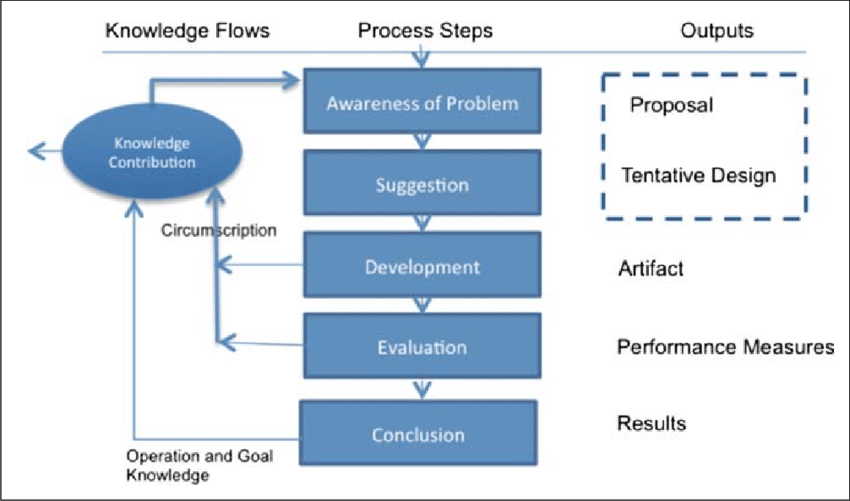
\includegraphics[width=\linewidth]{images/dsr.png}
    \caption{Design Science Research process (adapted from \citep{hevner2004design}).}
    \label{fig:dsr_methodology}
\end{figure}

The research was structured into five stages aligned with the \gls{dsr} cycle. Problem identification and threat analysis examined the \gls{mcp} specification to locate attack-surface expansion, trust boundaries, and protocol-level weaknesses, including \gls{threat_modeling} of client-server interactions, tool invocation, and agent-to-agent flows \citep{qi2025protocol}. The definition of security requirements then translated those weaknesses into functional and non-functional requirements that guide the architecture and establish measurable evaluation criteria \citep{nist2022ssdf, nist2020zerotrust}. Artifact design and development produced the tool itself, combining static analysis of server source, dynamic adversarial testing, testing of tool permission boundaries, and detection of potential data-leakage paths. Demonstration applies the artifact to controlled MCP environments and representative implementation scenarios, with adversarial cases simulating realistic attack patterns \citep{greshake2023prompt, owasp2024llm01}. Evaluation then assesses the tool against qualitative and quantitative criteria; this final stage is reported in Chapter~\ref{chap:results}.

\section{Document Structure}
\label{sec:structure}

The remainder of this dissertation is organized into five chapters. Chapter~\ref{chap:background} presents the theoretical framework, covering \glspl{llm}, the Model Context Protocol, and the cybersecurity concepts that underpin the work. Chapter~\ref{chap:architecture} describes the architecture of the proposed solution, including its two analysis paths, the shared taxonomy, and the main design decisions. Chapter~\ref{chap:implementation} details the implementation of each module. Chapter~\ref{chap:results} reports the evaluation, including the test targets, benchmarks, and a discussion of the results. Chapter~\ref{chap:conclusion} concludes and outlines directions for future work.

\chapter{Theoretical Framework}
\label{chap:background}

This chapter presents the theoretical foundations and state of the art related to \gls{mcp} and its security implications. It reviews \gls{mcp} architectures, adversarial risks, and existing research on securing tool-augmented and multi-agent \gls{ai} systems. Relevant methodologies and related studies are also discussed to establish the conceptual basis for the proposed tool.   

\section{Large Language Models and Agentic AI}
% TODO (this turn deferred by scope): expand this section.
% Cover: what an LLM is at the level this thesis needs (next-token prediction,
% instruction following, context window as the single trust-blind channel);
% the shift from a model that only emits text to an agent that calls tools and
% acts; why the inability to separate instructions from data in the context
% window is the root cause that the rest of the chapter builds on. Keep it short
% and in service of the security argument, not an LLM tutorial.
Large language models predict text from a context window that mixes system instructions, user input, and any external content retrieved at runtime. The model does not maintain a reliable boundary between these sources: an instruction embedded in retrieved data is read with the same weight as an instruction from the system prompt. When such a model is given the ability to invoke tools, it becomes an agent whose actions in the world are driven by that same undifferentiated context. This property is the root cause from which the attack surface discussed in the remainder of this chapter follows, and it is why defenses that assume a clean separation between trusted and untrusted input do not transfer directly to \gls{llm}-driven systems.

\section{Model Context Protocol and Agentic AI Architectures}

The \gls{mcp} enables large language models (\gls{llm}s) to interact with external tools, databases, and services through structured communication mechanisms \citep{anthropic2024mcp}. Unlike traditional \gls{ml} systems that operate within static inference environments, \gls{mcp}-based systems function as distributed, tool-augmented \gls{ai} architectures \citep{mitre2023atlas} in which language models may initiate external actions, retrieve contextual information, and collaborate with other agents.

From a systems perspective, \gls{mcp} introduces multiple execution layers and trust boundaries, as shown in Figure~\ref{fig:2}:

\newpage

\begin{figure}[htb]
    \centering
    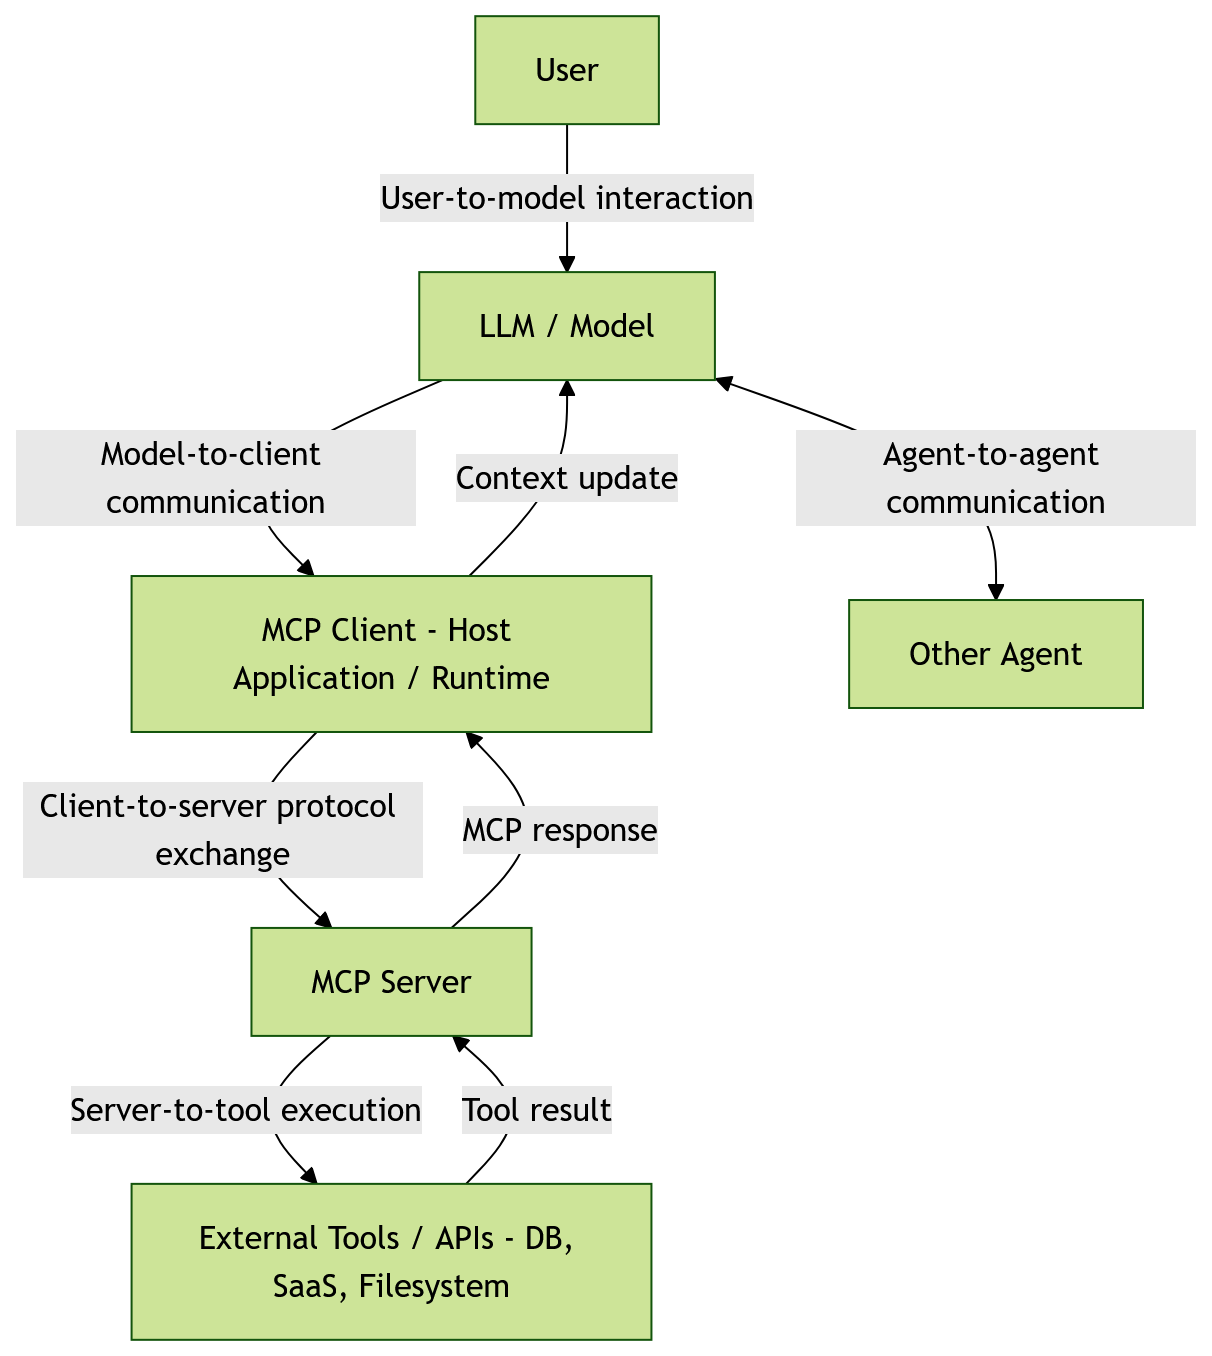
\includegraphics[width=0.8\linewidth]{images/mermaid-diagram-2026-02-23-233324.png}
    \caption{MCP Interactions Diagram}
    \label{fig:2}
\end{figure}

Each boundary represents a potential attack surface. In distributed systems theory, security risk increases with the number of interfaces and execution paths exposed to external input \citep{manadhata2011attack}. \gls{mcp} formalizes these interfaces and therefore structurally expands the attack surface of \gls{ai}-driven systems. This architectural shift necessitates security models that account for both protocol-level manipulation and semantic manipulation of model behavior.

\section{Attack Surface Expansion in Tool-Augmented LLM Systems}

Attack surface theory posits that the security exposure of a system grows as new interfaces, communication channels, and privilege domains are introduced \citep{manadhata2011attack, nist2022ssdf}. 
In \gls{mcp}-enabled environments, the attack surface expands along three principal dimensions:

\begin{enumerate}
    \item \textbf{External tool invocation} – \gls{llm}s are capable of triggering external tools based on natural language instructions. This introduces risks related to improper input validation, command injection, and unintended execution of sensitive operations. If tool interfaces are not strictly constrained, malicious or manipulated prompts may lead to unauthorized actions being performed at the system level.
 

    \item \textbf{Permission and authorization management} – MCP architectures rely on permission boundaries to control which tools and resources an agent can access. Weak or misconfigured access control mechanisms may allow privilege escalation, enabling agents to perform actions beyond their intended scope. Ensuring strict enforcement of least-privilege principles is therefore critical.

    \item \textbf{Multi-agent communication flows} – In systems involving \gls{a2a} communication, agents exchange information and delegate tasks. This introduces risks such as trust boundary violations, propagation of malicious instructions across agents, and cascading compromise scenarios where a single compromised agent affects the entire system.
\end{enumerate}

Unlike traditional web applications, \gls{mcp} systems combine probabilistic reasoning (\gls{llm} inference) with deterministic execution (tool invocation). This hybrid execution model creates a class of vulnerabilities in which semantic manipulation through natural language may result in concrete system-level actions \citep{greshake2023prompt, mitre2023atlas}. Therefore, \gls{mcp} security must be analyzed not only through classical input validation models but also through adversarial reasoning tools. Some \gls{mcp} systems may also involve contextual data retrieval mechanisms, which can introduce additional security considerations; however, this aspect is outside the scope of this work.

\section{Adversarial Machine Learning and Prompt Injection}

Adversarial \gls{ml} provides the theoretical foundation for understanding how \gls{ai} systems can be manipulated through crafted inputs. In \gls{llm}-based architectures, adversarial behavior most commonly manifests as \gls{prompt_injection}.

Prompt injection exploits the model’s reliance on contextual instructions \citep{greshake2023prompt, liu2024universal}, attempting to override system-level constraints or introduce malicious operational directives. In \gls{mcp} environments, such attacks may induce:

\begin{itemize}
    \item Unauthorized tool execution,
    \item Privilege escalation,
    \item Data exfiltration,
    \item Cross-agent contamination.
\end{itemize}

These attack vectors are particularly challenging to mitigate due to the probabilistic nature of \gls{llm} behavior. Unlike traditional software systems, where execution paths are explicitly defined, \gls{llm}s interpret instructions based on contextual understanding, making it difficult to enforce strict separation between trusted and untrusted inputs \citep{greshake2023prompt, liu2024universal}.

Furthermore, prompt injection can be indirect, where malicious instructions are embedded in external data sources such as web pages, documents, or database entries retrieved at runtime. This significantly broadens the threat landscape, as attackers do not need direct access to the system prompt to influence model behavior.

As a result, effective mitigation requires a combination of techniques, including input sanitization, contextual isolation, permission-aware execution, and continuous adversarial testing. These approaches shift security from purely preventive mechanisms to adaptive and resilience-based strategies.

Theoretical work on adversarial robustness demonstrates that language models cannot reliably distinguish between benign and malicious instructions embedded within contextual data. Consequently, defense strategies must rely on architectural safeguards, permission enforcement, validation layers, and adversarial testing rather than purely on model alignment techniques.

\section{Threat Modeling in Protocol-Driven AI Systems}

\gls{threat_modeling} is a structured methodology for identifying and categorizing vulnerabilities across system components and trust boundaries. In distributed and protocol-driven systems, methodologies such as STRIDE (Spoofing, Tampering, Repudiation, Information Disclosure, Denial of Service, Elevation of Privilege) provide systematic coverage of security risks \citep{mitre2023atlas}.

This implies that threat modeling must consider not only classical vulnerabilities but also how contextual inputs can influence system behavior. For example, a seemingly benign prompt may lead to unintended tool execution if the model misinterprets intent or if safeguards are insufficient.


Applying threat modeling to \gls{mcp} involves analyzing:

\begin{itemize}
    \item Authentication and identity validation between client and server,
    \item Integrity of contextual payloads,
    \item Confidentiality of retrieved resources,
    \item Authorization boundaries governing tool execution,
    \item Lateral movement across agents in \gls{a2a} scenarios.
\end{itemize}

Formal threat modeling enables classification of vulnerabilities and supports the design of automated detection mechanisms. This theoretical foundation directly informs the development of the \gls{mcp} security scanning agent proposed in this research.

\section{Automated Vulnerability Detection and Continuous Validation}

Modern cybersecurity practice relies on automated vulnerability detection mechanisms, combining static analysis, dynamic testing, and adversarial simulation \citep{owasp2025thirdparty, owasp2024llm01}.

\gls{static_analysis} enables detection of structural weaknesses in source code, such as improper permission handling or insecure token validation. \gls{dynamic_testing} evaluates runtime behavior under controlled adversarial conditions.

In addition to traditional techniques, MCP security requires \textbf{semantic adversarial testing}, where malicious or crafted prompts are systematically generated to evaluate how \gls{llm}-driven systems respond to adversarial inputs. This form of testing targets vulnerabilities that arise from the interpretation of natural language, including \gls{prompt_injection}, context manipulation, and unintended action triggering \citep{greshake2023prompt, liu2024universal}.


Continuous validation aligns with \gls{defense_in_depth} theory \citep{nist2022ssdf}, which advocates layered security mechanisms rather than reliance on a single control. Integrating automated security scanning into development pipelines allows \gls{mcp} implementations to be re-evaluated not only at design time but also later in their lifecycle.


Together, these foundations justify the development of a secure development and testing tool for \gls{mcp} implementations and provide the conceptual basis for the automated \gls{mcp} security scanning agent proposed in this dissertation.
\chapter{Solution Architecture}
\label{chap:architecture}

% =====================================================================
%  Chapter 3 with glossary/acronym cross-references wired in.
%  Acronyms: \gls{} on first prose use (auto-expands), \acrshort{} in
%  tables (short form, no expansion). Glossary terms: \gls{} / \glsdisp{}.
%  Requires the entries from chap3-additions.tex to be present in
%  acronimos.tex and glossario.tex, otherwise these keys are undefined.
% =====================================================================

This chapter describes the architecture of the proposed tool. It presents the two complementary analyses the tool performs, the shared vocabulary that ties their results together, the decomposition into components, the data that moves between them, and the architectural decisions that a reviewer is most likely to question. Implementation detail, meaning how each component is actually built, is deferred to Chapter~\ref{chap:implementation}; this chapter stays at the level of structure and rationale.

\section{Overview}

The tool answers a single question, ``how secure is this \gls{mcp} server,'' along two paths that are useful in different situations. The first is a \emph{dynamic} analysis: it connects to a running server, reasons about the tools the server exposes, and sends real attack traffic to find out which of those tools actually leak or misbehave. The second is a \emph{static} analysis: it reads a server's source code and flags the code that would answer those same attacks, without connecting to anything or executing a single line.

The two paths are deliberately built on one foundation. Both label every finding with the same vulnerability taxonomy (Section~\ref{sec:taxonomy}) and draw remediation text from the same catalog. A finding of type \texttt{command\_injection} therefore means the same thing whether it came from a payload that succeeded against a live server or from a line of source code that a parser flagged. This shared vocabulary is what lets a developer fix statically what the dynamic path would otherwise prove the hard way, and it is the single most important structural property of the design.

\section{The Dynamic Scan Pipeline}
\label{sec:pipeline}

The dynamic path is a seven-step pipeline, shown in Figure~\ref{fig:pipeline}. The steps fall into two groups separated by a human decision, and that separation is a security property of the architecture rather than a convenience of the user interface.

\begin{figure}[htbp]
    \centering
    % TODO: export images/arch-pipeline.svg to images/arch-pipeline.pdf
    % (Overleaf: upload the .svg and it is converted on compile; locally use
    %  Inkscape or rsvg-convert. The .svg source is already in images/.)
    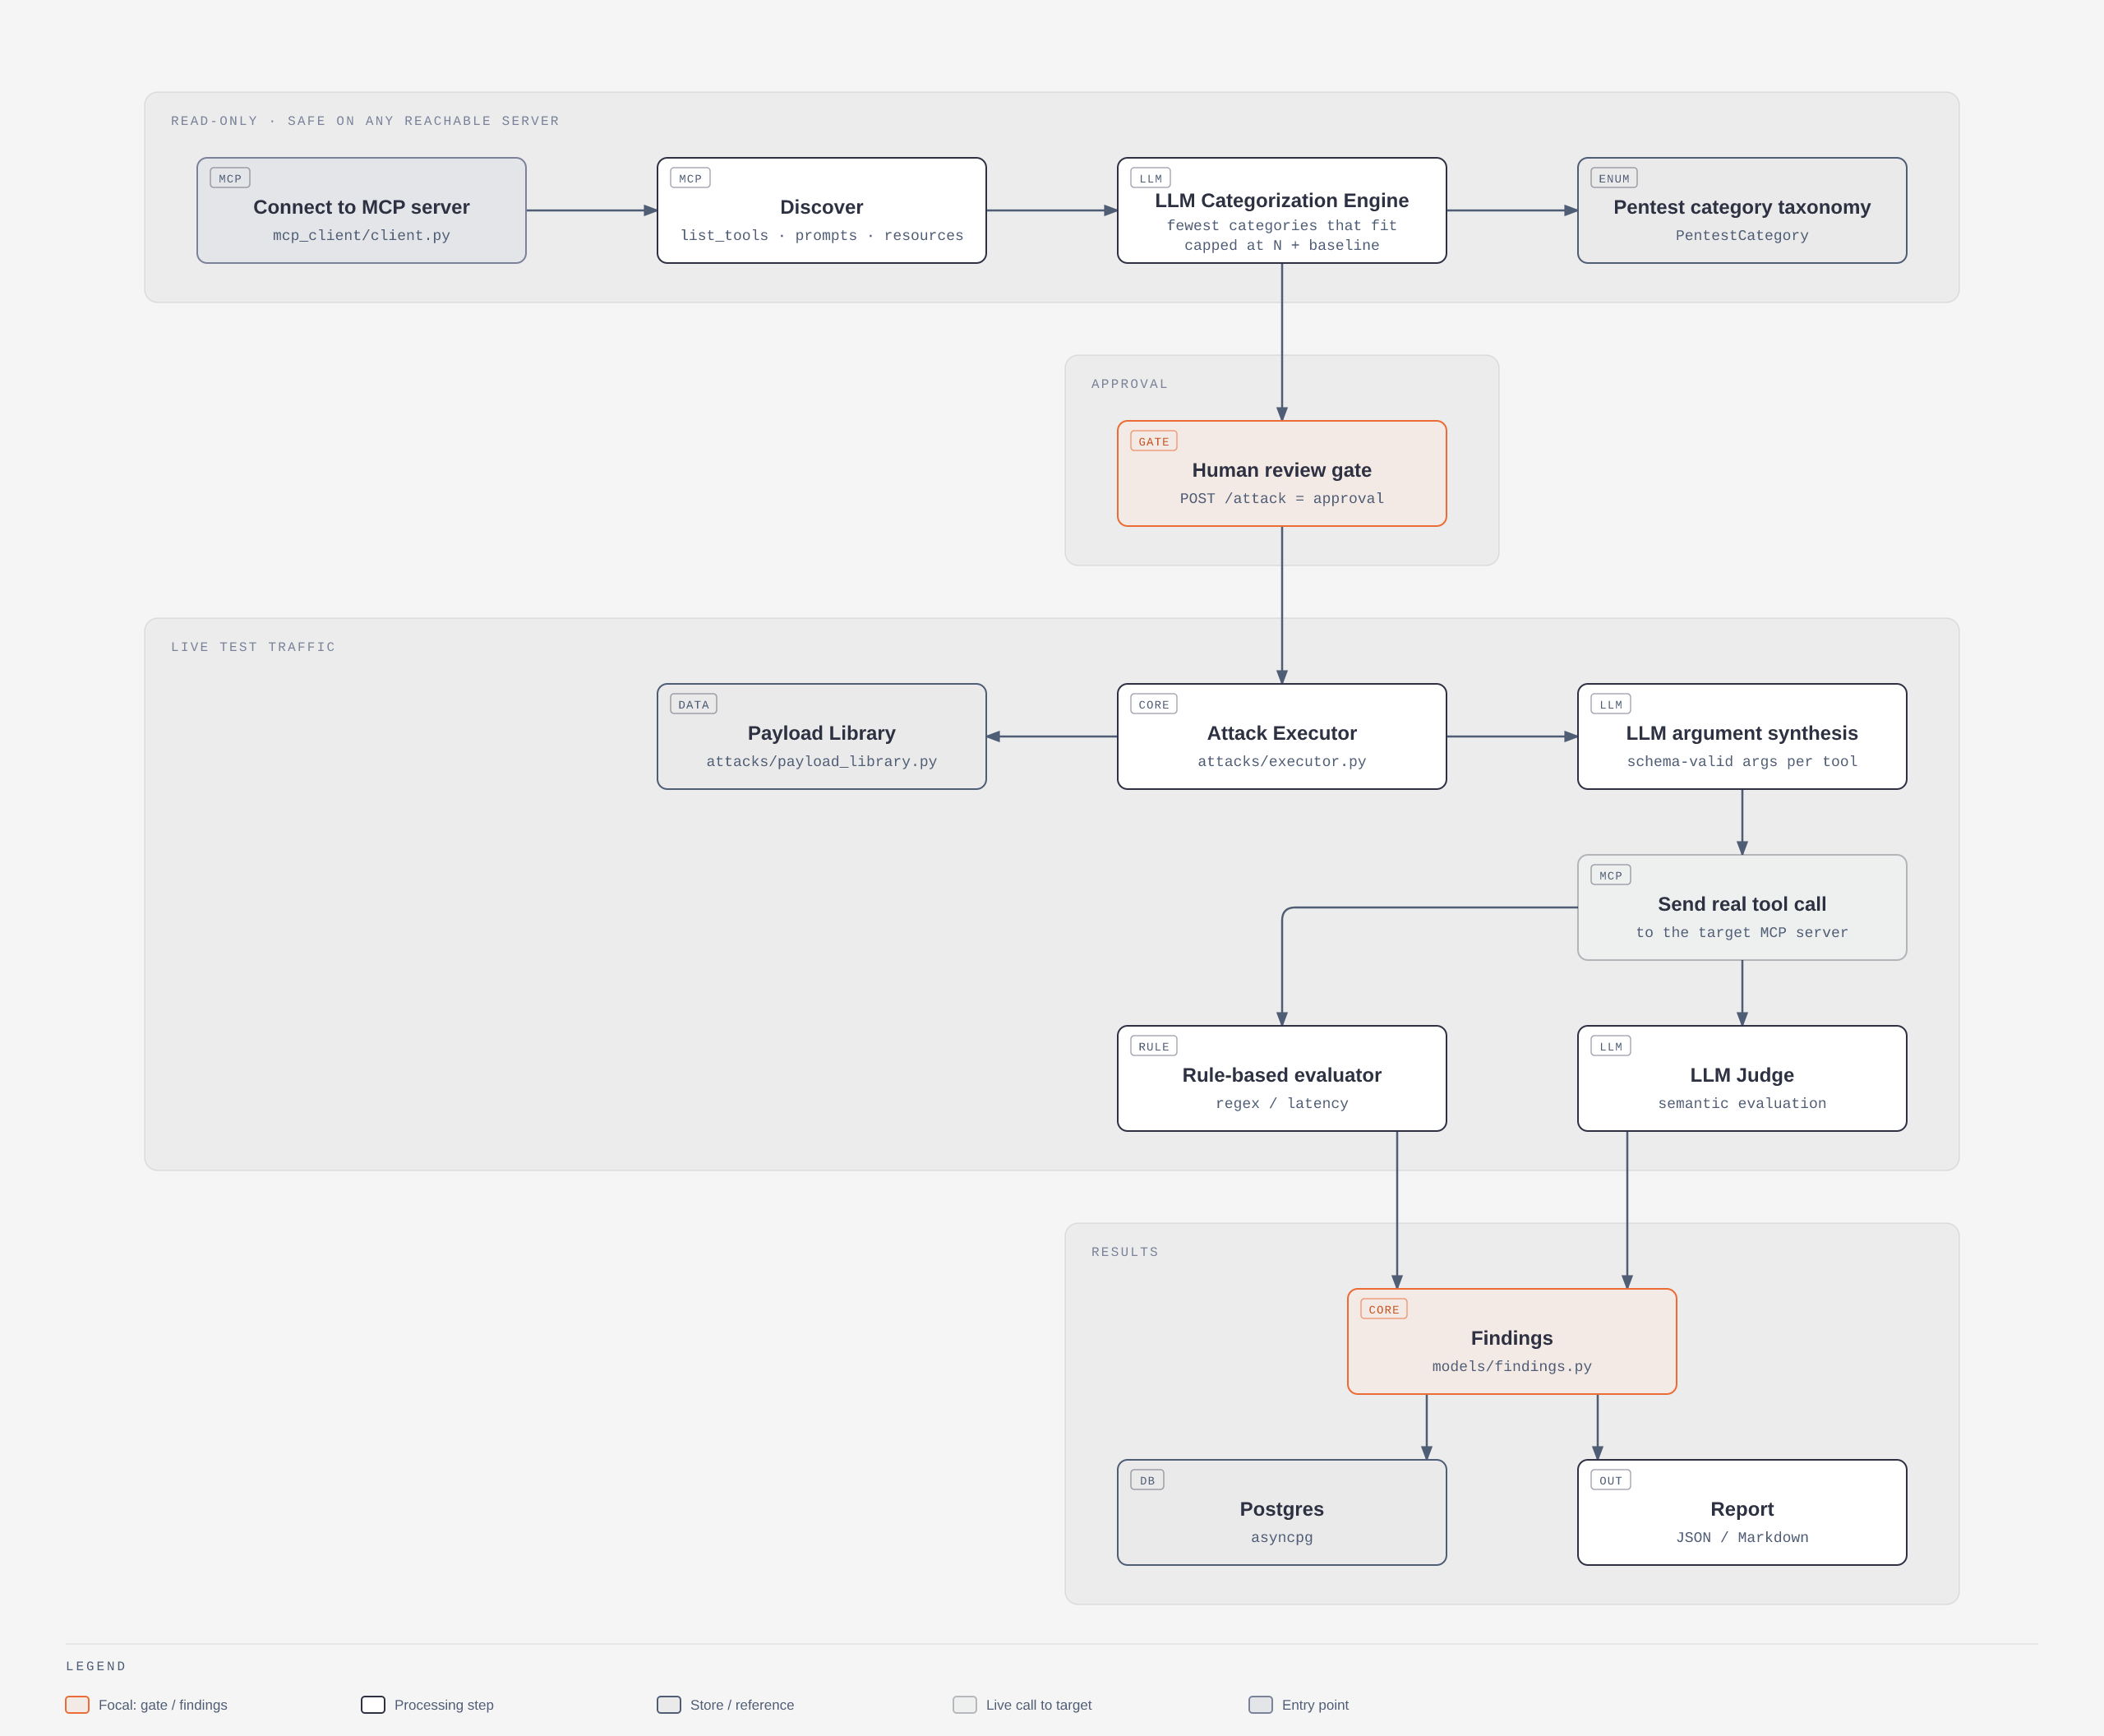
\includegraphics[width=\linewidth]{images/arch-pipeline.png}
    \caption{The dynamic scan pipeline. Steps 1--3 are read-only; steps 5--7 send live attack traffic and run only after an explicit approval.}
    \label{fig:pipeline}
\end{figure}

The first group discovers and understands the target without touching it in anger. The tool connects to the \gls{mcp} server over one of the protocol's transports, calls the server's own listing methods to enumerate the tools, prompts, and resources it exposes, and then classifies each discovered tool. Classification is where a language model first enters the pipeline. A System One model, Jev (Section~\ref{sec:system-one}), reads each tool's name, description, and input schema and answers one independent yes/no question per category, returning the probability that the category is the tool's primary attack surface. The application keeps only the categories above a probability threshold, at most one per tool in the current configuration, so a plainly database-backed tool is not tagged with a spread of speculative categories that would each multiply the attacks sent. Everything up to this point is read-only and safe to run against any reachable server.

Between understanding and attacking sits a \glsdisp{human_in_the_loop}{human-in-the-loop} gate. The categorization is returned to the operator for inspection, and nothing is attacked until the operator explicitly approves. This gate is not cosmetic: it is the boundary at which the tool stops being an observer and starts sending traffic that could cause real effects, and the architecture makes that boundary an explicit, separate action.

The second group tests and reports. For each approved combination of tool, category, and payload, the \gls{llm} synthesizes a schema-valid call that places the attack \gls{payload} in the field most likely to reach a vulnerable \gls{sink} while filling every other required field with a plausible benign value. Each response is then evaluated twice. Fast deterministic rules catch known-format leaks such as secrets, stack traces, or \glsdisp{canary_string}{canary strings}, and an \gls{llm} judge catches the leaks that only semantic understanding can recognize, such as a response that returned another tenant's record. The judge is required to quote the exact span of the response that proves the leak, and the tool verifies that quote is present before trusting the verdict. Finally, the confirmed findings are assembled into a structured report. Each finding carries a \gls{cvss} v3.1 base score and severity band, its impact on confidentiality, integrity, and availability, the judge's confidence, the evidence, and the exact payload used.

\newpage

\section{Vulnerability Taxonomy}
\label{sec:taxonomy}

The taxonomy is the shared vocabulary named in the overview. It extends a small set of initial categories into a fuller set aligned with the \gls{owasp} Top 10 for \gls{llm} Applications and the MITRE \gls{atlas} mappings established in the project's earlier research phase, so a finding here cites the same external framing used elsewhere. Table~\ref{tab:taxonomy} lists the categories and what each one looks for.

\begin{table}[htbp]
\centering
\small
\begin{tabular}{p{4.2cm} p{8.0cm}}
\hline
\textbf{Category} & \textbf{What it looks for} \\
\hline
\acrshort{sql} Injection & Parameters that build or forward a database query \\
\gls{command_injection} & Parameters that reach a shell or subprocess \\
\gls{path_traversal} & File-path parameters on read/write/list/delete tools \\
\acrshort{ssrf} & \acrshort{url} or host parameters that trigger outbound requests \\
Information Extraction & Responses containing secrets, credentials, or internal metadata \\
Resource Extraction & Over-broad or cross-tenant resource exposure \\
\gls{jailbreak} / \gls{prompt_injection} & Tools that process natural-language or instruction text \\
Auth \& Access Control & Privileged-sounding tools, tested under a low-privilege session \\
\glsdisp{deserialization_attack}{Deserialization} & Parameters parsed as \acrshort{json}, \acrshort{yaml}, or pickled data \\
Memory \& Persistence Poisoning & Writes to stores read back in a different session \\
\acrshort{dos} / Resource Exhaustion & Unbounded or expensive operations \\
Generic Schema \glsdisp{fuzzing}{Fuzzing} & Applied to every tool as the baseline floor \\
\hline
\end{tabular}
\caption{The pentest category taxonomy shared by the dynamic and static paths.}
\label{tab:taxonomy}
\end{table}

One category, generic schema fuzzing, is a non-negotiable floor. Every tool receives it regardless of what the classifier decides, which matters because a tool description is untrusted content that an attacker could craft to talk the classifier out of flagging anything. The floor guarantees that every tool is attacked at a baseline level even if the classifier is manipulated, fails, or times out. The rationale for this floor as a defense against injection aimed at the tool's own triage step is examined in Section~\ref{sec:decisions}.

\subsection{Severity Scoring}
\label{sec:scoring}

A finding has to say how serious it is and what it puts at risk. Rather than define a project-specific scale, the tool adopts the \gls{cvss} v3.1 base metrics~\cite{first2019cvss}. The choice has two practical consequences. First, the confidentiality, integrity, and availability triad is already part of every \gls{cvss} vector as the C, I, and A impact metrics, so the \gls{cia} impact of a finding is read directly from the same vector that produces its score. Second, the 0 to 10 number and its band (None, Low, Medium, High, Critical) are computed by the standard's published formula, so no score in the report is chosen by hand.

Each category in the taxonomy is assigned one base vector, stored next to its remediation text in the shared catalog. All vectors assume an \gls{mcp} server reachable over the network by an unauthenticated caller (AV:N, PR:N, UI:N) unless the category itself implies otherwise. Table~\ref{tab:cvss} lists the vectors and the resulting scores.

\begin{table}[htbp]
\centering
\small
\begin{tabular}{p{4.0cm} p{4.6cm} c c c}
\hline
\textbf{Category} & \textbf{Base vector (after \texttt{CVSS:3.1/})} & \textbf{Score} & \textbf{Band} & \textbf{C/I/A} \\
\hline
Command Injection & \texttt{AV:N/AC:L/PR:N/UI:N/S:C/C:H/I:H/A:H} & 10.0 & Critical & H/H/H \\
SQL Injection & \texttt{AV:N/AC:L/PR:N/UI:N/S:U/C:H/I:H/A:L} & 9.4 & Critical & H/H/L \\
SSRF & \texttt{AV:N/AC:L/PR:N/UI:N/S:C/C:H/I:L/A:N} & 9.3 & Critical & H/L/N \\
Jailbreak / Prompt Injection & \texttt{AV:N/AC:L/PR:N/UI:N/S:C/C:L/I:H/A:N} & 9.3 & Critical & L/H/N \\
Memory \& Persistence Poisoning & \texttt{AV:N/AC:L/PR:N/UI:N/S:C/C:L/I:H/A:N} & 9.3 & Critical & L/H/N \\
Path Traversal & \texttt{AV:N/AC:L/PR:N/UI:N/S:U/C:H/I:L/A:N} & 8.2 & High & H/L/N \\
Auth \& Access Control & \texttt{AV:N/AC:L/PR:L/UI:N/S:U/C:H/I:H/A:N} & 8.1 & High & H/H/N \\
Deserialization & \texttt{AV:N/AC:H/PR:N/UI:N/S:U/C:H/I:H/A:H} & 8.1 & High & H/H/H \\
Information Extraction & \texttt{AV:N/AC:L/PR:N/UI:N/S:U/C:H/I:N/A:N} & 7.5 & High & H/N/N \\
DoS / Resource Exhaustion & \texttt{AV:N/AC:L/PR:N/UI:N/S:U/C:N/I:N/A:H} & 7.5 & High & N/N/H \\
Resource Extraction & \texttt{AV:N/AC:L/PR:L/UI:N/S:U/C:H/I:N/A:N} & 6.5 & Medium & H/N/N \\
Generic Schema Fuzzing & \texttt{AV:N/AC:L/PR:N/UI:N/S:U/C:N/I:L/A:L} & 6.5 & Medium & N/L/L \\
\hline
\end{tabular}
\caption{\gls{cvss} v3.1 base vector, score, band, and \gls{cia} impact per taxonomy category.}
\label{tab:cvss}
\end{table}

The metric choices that move the score most deserve a justification. Scope is set to changed (S:C) where a successful attack reaches a component beyond the \gls{mcp} server itself: command injection escapes into the host operating system, \gls{ssrf} reaches internal services behind the server, and prompt injection and memory poisoning alter the behaviour of the \gls{llm} agent that consumes the tool's output. Availability is high (A:H) for resource exhaustion, whose whole effect is denial of service, and for command injection and deserialization, where arbitrary code execution can stop the process. Deserialization is the only category with high attack complexity (AC:H), because exploiting it generally requires a gadget chain that matches the target's libraries; this is why it scores below path traversal despite a high impact on all three properties. Resource extraction and access-control failures require low privileges (PR:L), since both describe an authenticated caller reaching data beyond its own. Generic schema fuzzing carries only low integrity and availability impact, because a fuzzing hit shows that malformed input is mishandled but does not by itself demonstrate a leak.

These vectors are a defensible starting point, not fixed truths, and they are kept as data in the catalog so they can be revised without touching code.


\section{The Static Analysis Path}
\label{sec:static}

The static path reads source code and never connects to a server. It walks a checkout for Python files, parses each one, inventories what the server exposes, and flags the code an attacker could reach. The inventory records server instantiation, the tool, resource, and prompt registrations with their parameters and line ranges, the declared transport, and any authentication hints. Risk detection then runs over the same files and keeps only the findings that map onto the taxonomy, attributing each one to the specific tool whose body contains it. A dangerous call inside a registered tool is reachable by anything that can invoke that tool; the same call in a helper script is not, and the attribution preserves that distinction.

The two paths exist together because they answer different questions about the same weakness, as Table~\ref{tab:static-vs-dynamic} sets out. The static path answers ``which code would answer this payload,'' with a line of source as evidence, before the dynamic path, or anyone else's pentest tool, answers ``did this payload actually work'' with the server's response as evidence.

\begin{table}[htbp]
\centering
\small
\begin{tabular}{p{3.2cm} p{4.6cm} p{4.6cm}}
\hline
 & \textbf{Dynamic scan} & \textbf{Static analysis} \\
\hline
Needs & Running server and credentials & A source checkout \\
Sends attack traffic & Yes, after the human gate & Never \\
Answers & ``Did this payload work?'' & ``Which code answers it?'' \\
Evidence & The server's response & The line of code \\
\hline
\end{tabular}
\caption{The two analysis paths answer different questions over the same taxonomy.}
\label{tab:static-vs-dynamic}
\end{table}

\section{Component Architecture}
\label{sec:components}

Figure~\ref{fig:components} shows the decomposition into components. At the centre is a set of data models that form the shared vocabulary every other component speaks: a normalized representation of a discovered tool, the categorization result, the synthesized attacks and their verdicts, and the final report. Keeping these models in one place is what allows the dynamic and static paths to produce comparable output without coordinating directly.

\begin{figure}[htbp]
    \centering
    % TODO: export images/arch-components.svg to images/arch-components.pdf
    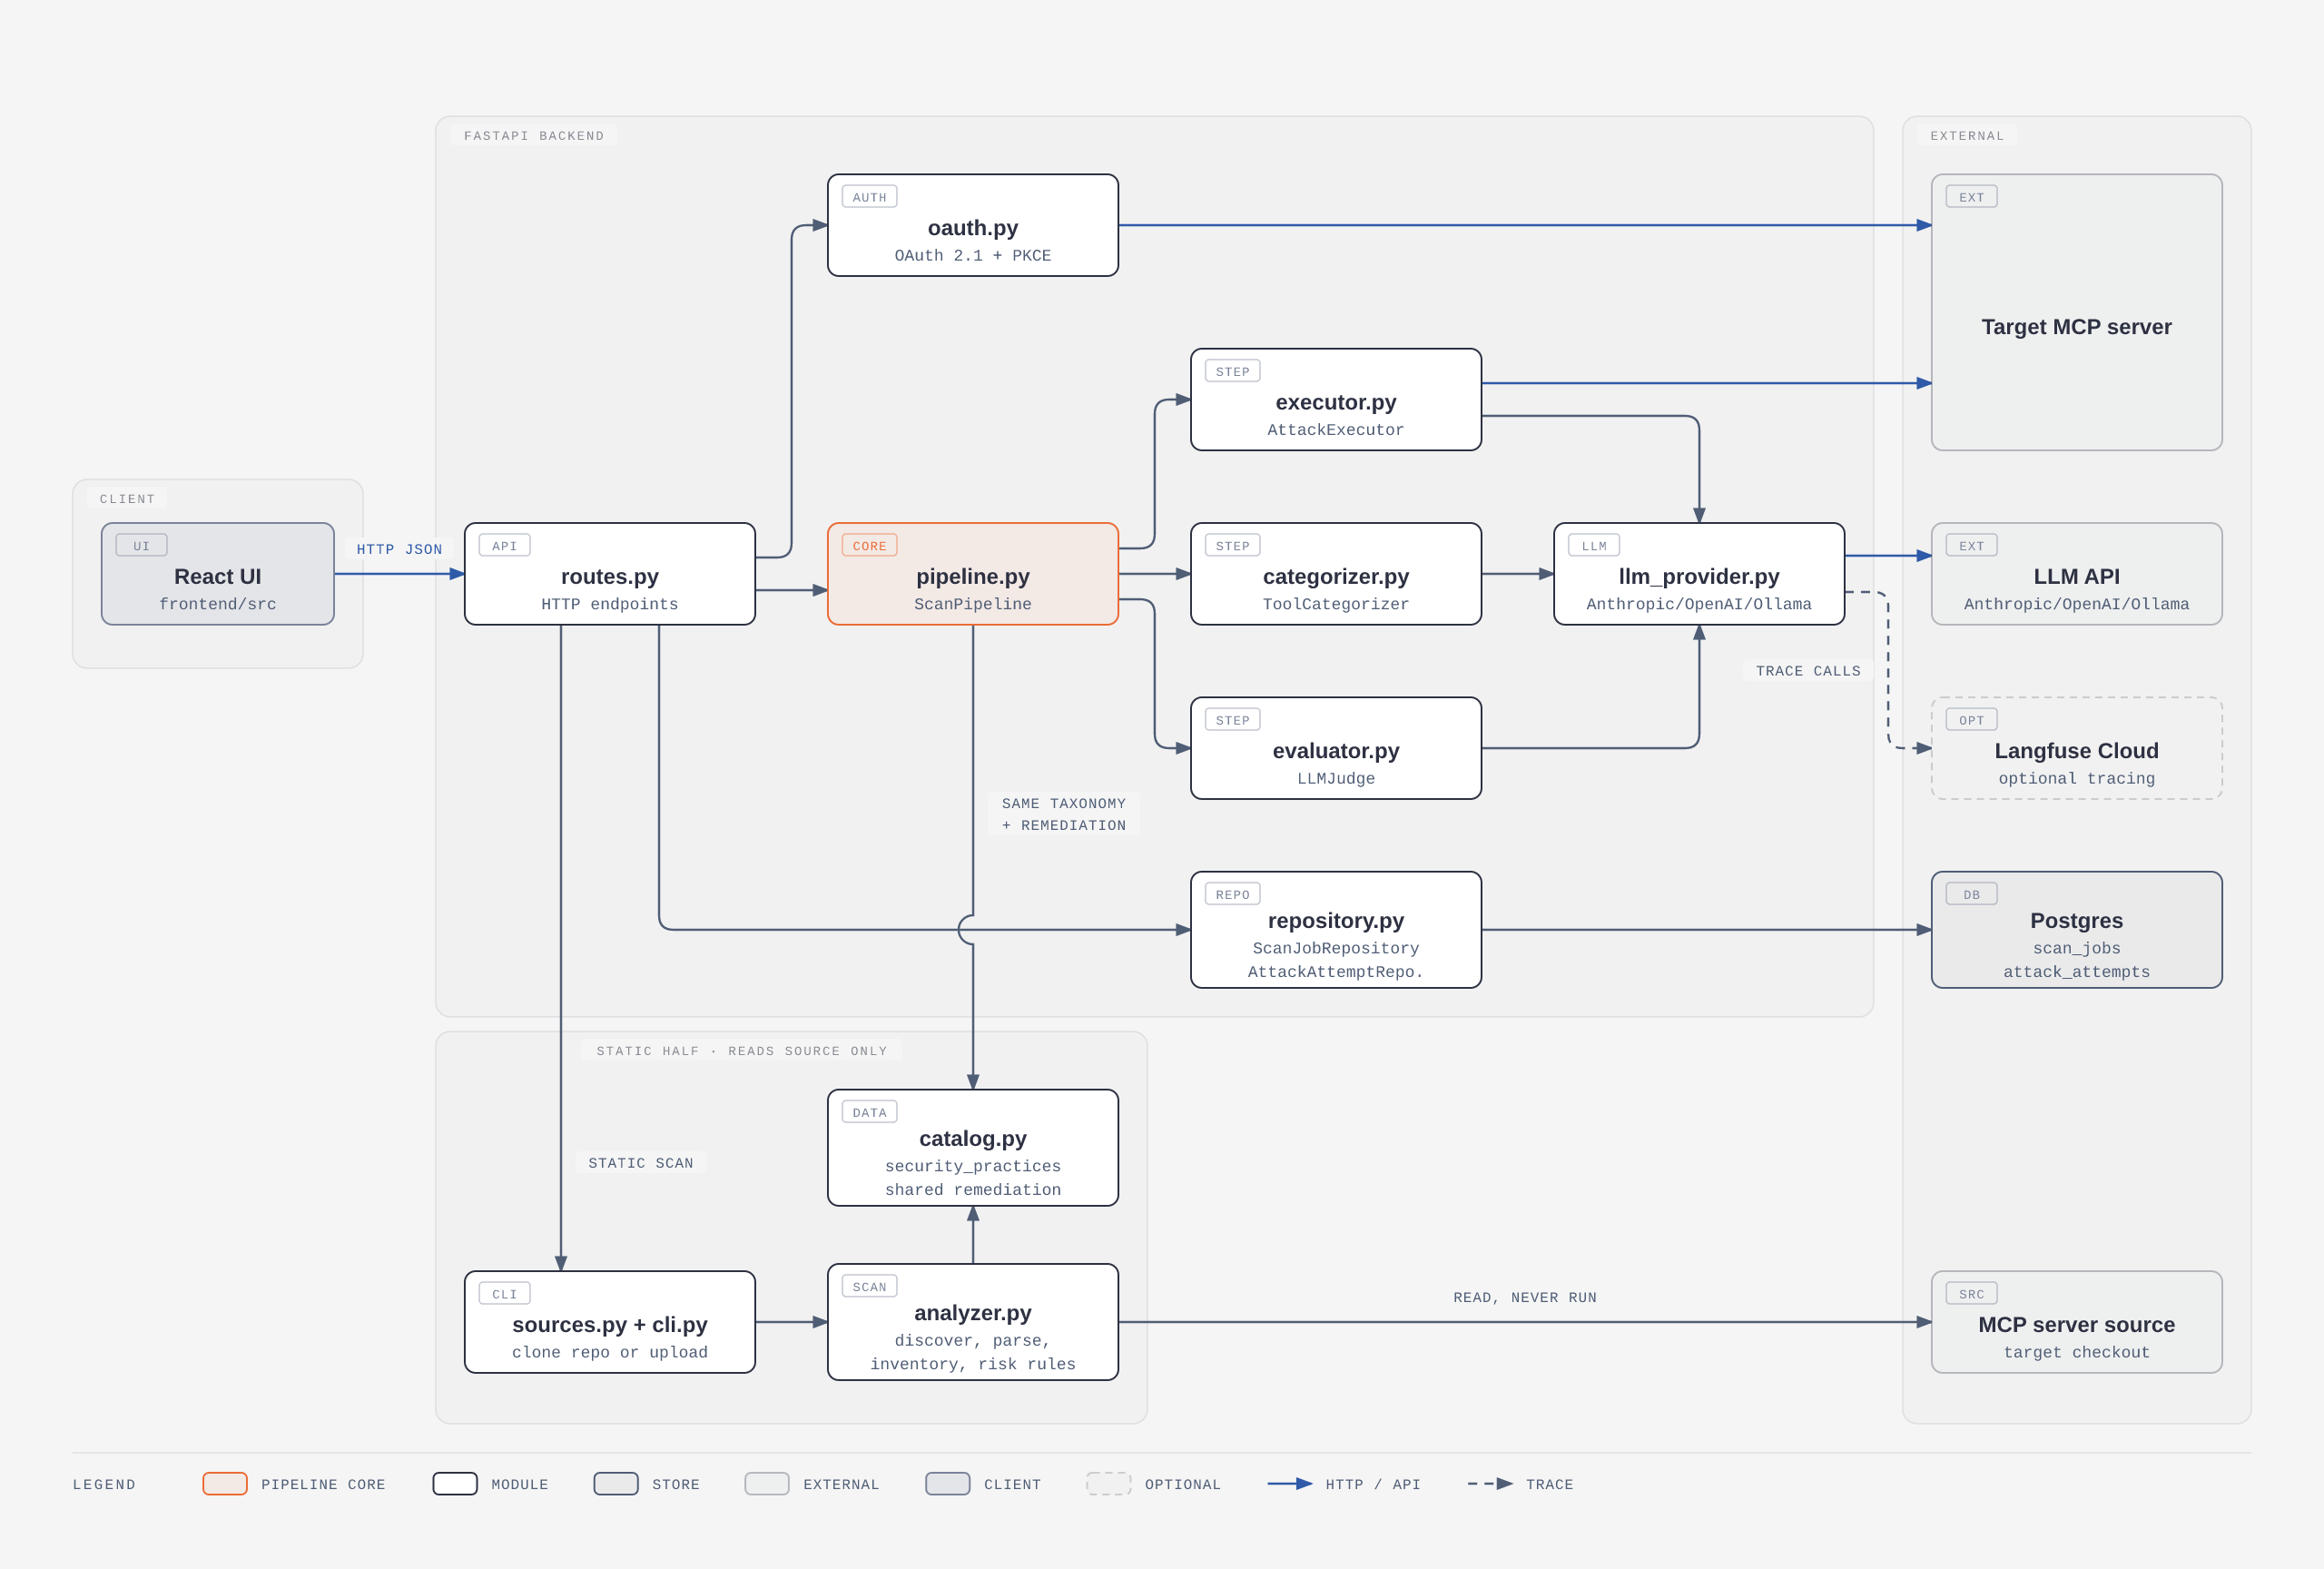
\includegraphics[width=\linewidth]{images/arch-components.png}
    \caption{Component decomposition. The shared data models sit between the two analysis paths.}
    \label{fig:components}
\end{figure}

Around that core, the dynamic path is built from an \gls{mcp} client that handles the three transports, a connection layer that owns credential lifecycle and the \gls{oauth} flow, a categorization component that calls the Jev \gls{api}, an \gls{llm} provider component shared by attack synthesis and judging, an attacks component that holds the payload library and the synthesis logic, an evaluation component that runs the dual verdict, and an orchestration layer that wires these together and owns the human-approval split. The static path is a self-contained set of components for obtaining source, walking it safely, parsing it, inventorying the exposed surface, and running the risk rules. Supporting both are a security-practices catalog that supplies remediation, a persistence layer that is the only code allowed to touch the database, a reporting component, and the web \gls{api}. A React frontend presents the whole as three tabs: the live-scan wizard, the payload library and attack history, and the code-review view.

\section{Data Model and Persistence}
\label{sec:data}

Figure~\ref{fig:data-model} shows the persisted data model. The design records the \emph{outputs} of a scan, the snapshot of what the server exposed, the categorization, and the report, and stores them in a relational database using \acrshort{json} columns so that these evolving structures do not require a rigid schema this early in the project. Durable scan history is what gives the tool value a single-shot scanner lacks: the ability to compare a server against itself over time.

\begin{figure}[htbp]
    \centering
    % TODO: export images/arch-data-model.svg to images/arch-data-model.pdf
    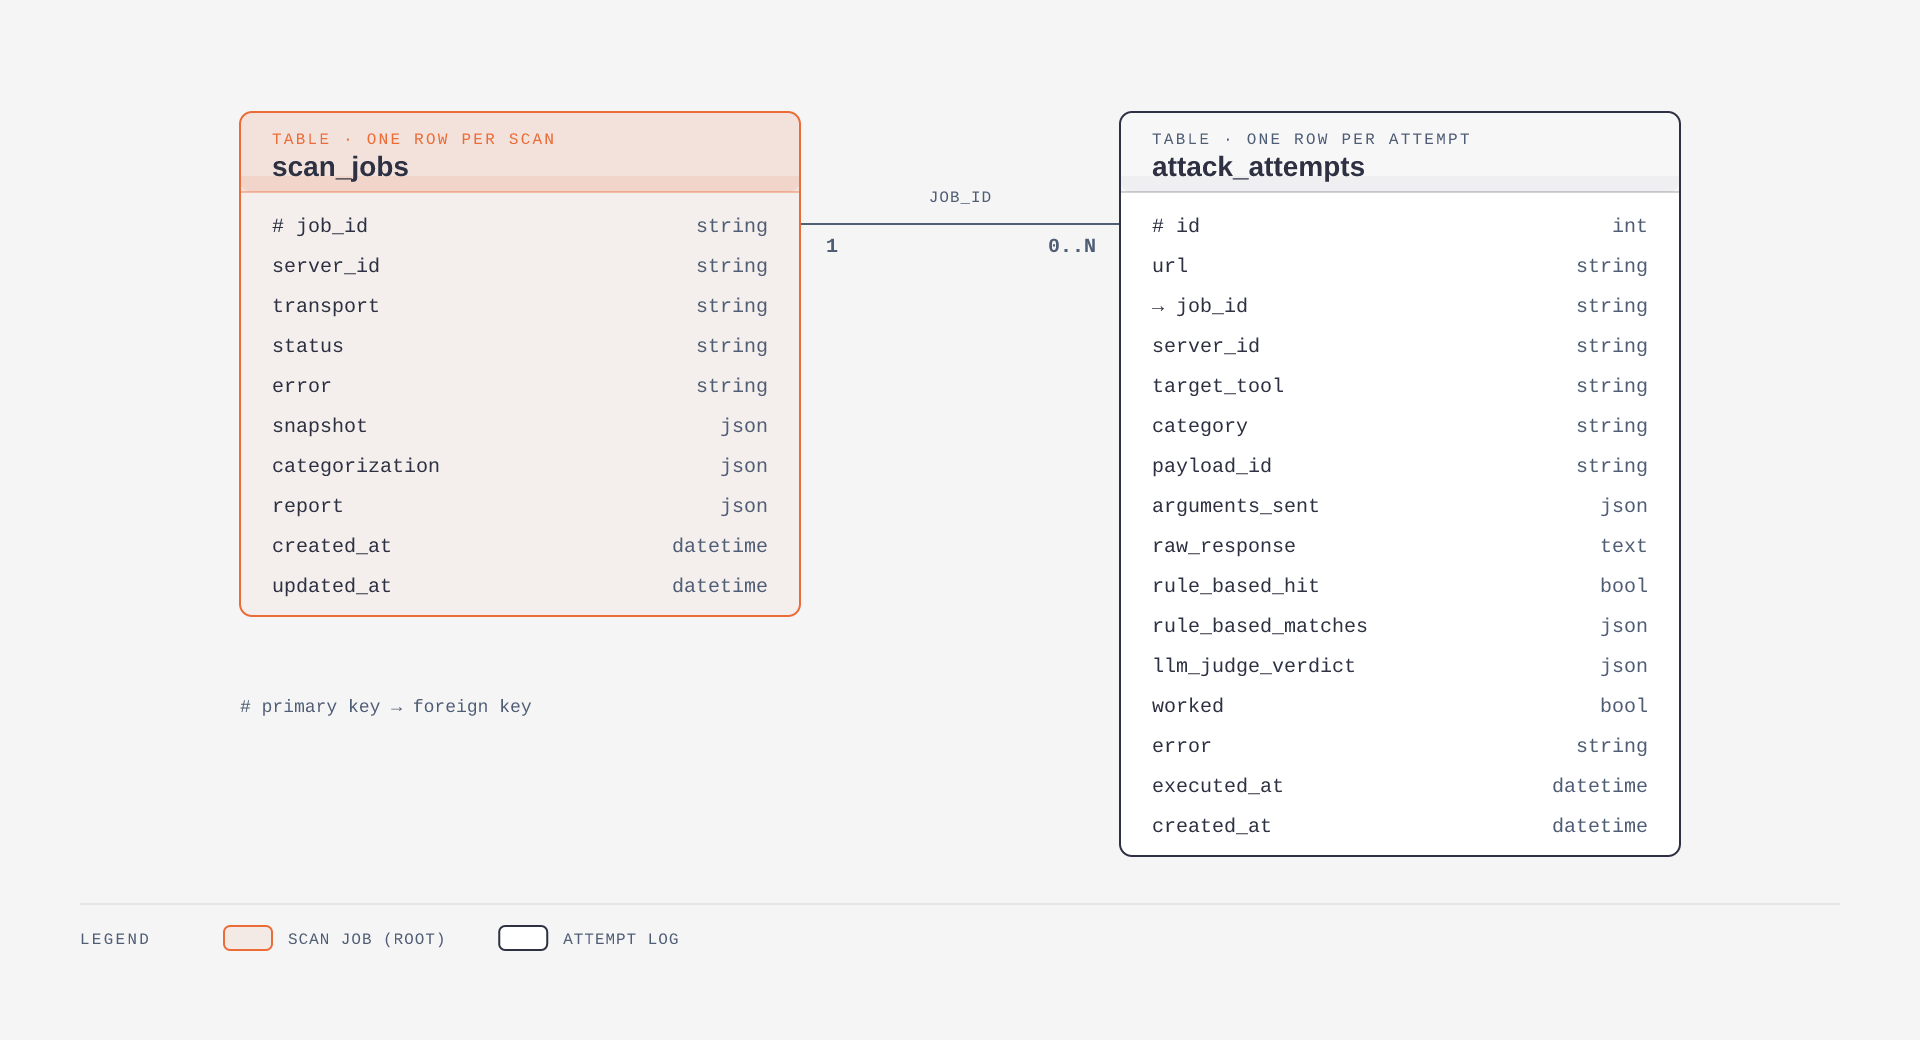
\includegraphics[width=\linewidth]{images/arch-data-model.png}
    \caption{Persisted data model. Only scan outputs are stored; connection credentials never are.}
    \label{fig:data-model}
\end{figure}

What the model deliberately does not store is the connection credentials. The \acrshort{url}, headers, or command used to reach the target, which may carry a bearer token for the server under test, live only in memory for the duration of one discover-then-attack cycle and are deleted as soon as the attack run finishes. The cost of this choice is that a process restart between discovery and attack forces a fresh discovery; the benefit is that a security tool never becomes a store of the very credentials it was handling. This is examined further in the next section.

\section{Architectural Design Decisions}
\label{sec:decisions}

Several choices shape the architecture rather than any single component, and each answers a question a reviewer would reasonably raise.

Discovery and attack are two separate operations. The read-only discovery call never sends attack traffic, and the attack call refuses to run without the identifier of a prior discovery. This is the structural form of the \glsdisp{human_in_the_loop}{human-in-the-loop} gate: nothing is attacked without a deliberate second action, taken after the operator has seen the full categorization.

Connection credentials are never persisted. As described in Section~\ref{sec:data}, only scan outputs reach the database. For a security tool specifically, the risk of accumulating target credentials outweighs the convenience of surviving a restart.

Evaluation is dual rather than single. Rule-based checks are fast, precise, and free, but blind to anything that does not match a known format. The \gls{llm} judge catches the semantic leaks no regular expression could enumerate in advance, at the cost of one extra model call, and it runs only where that cost is justified. Crucially, the judge's verdict is grounded, not trusted: it must quote the exact span of the response that proves the finding, and a verdict whose evidence cannot be located in the response is overruled. This guard is deterministic and independent of which model is configured, so it catches a confidently wrong judge regardless of provider.

Severity comes from a public standard rather than from the judge. The \gls{llm} judge decides whether an attack succeeded and how confident it is, but the severity of a confirmed finding is the band of its category's \gls{cvss} vector (Section~\ref{sec:scoring}). Letting the model also choose the severity would put a second unvalidated judgement in the report, one that could differ between runs and providers for the same evidence. Fixing it to the standard makes every finding of the same category comparable across servers, scans, and models. The same reasoning sets the single aggregate figure for a scan: the highest \gls{cvss} score among its findings, which is the usual convention in vulnerability reporting: the worst confirmed weakness decides how exposed the server is.


Classification uses a System One model rather than a generative \gls{llm}. The tool was first built with an \gls{llm} classifier, which is kept in the code for comparison. Classification is a narrow decision, repeated for every tool and category and consumed by code rather than read by a person, which is the case a System One model is built for: each category becomes an independent probability that can be thresholded, instead of a list the model writes and the code must parse. In a benchmark over the 22 tools of the evaluation corpus (Chapter~\ref{chap:results}), Jev reached an F1 score of 0.86, against 0.84 and 0.86 for the \gls{llm} classifier (GPT-5.4 mini) in two runs, at roughly one seventh of the cost and less than half of the latency per tool. Attack synthesis and judging stay with a generative \gls{llm}, because they require writing text and explaining a verdict.

The classifier has a floor it cannot remove. Because a tool description is untrusted text fed into a model, a crafted description could try to manipulate the classifier into reporting nothing. Each Jev question therefore instructs the model to treat the tool definition as data rather than instructions, the application adds the generic-fuzzing floor to every result whatever the model answers, and a tool whose classification fails falls back to that baseline instead of being dropped. Together these ensure that no tool silently vanishes from the results. The tool's own triage step is exposed to the same injection risk it is built to detect, and the architecture answers that explicitly rather than assuming the classifier is trustworthy.

Attacks run sequentially by default. A strictly sequential run is deterministic and reproducible, which is the right baseline for any measurement. Parallelism is available on request for speed, but it changes the order and the load, not the set of findings, and timing-sensitive checks are always isolated so that scan-induced load cannot corrupt a latency-based verdict.

\chapter{Implementation}
\label{chap:implementation}


This chapter describes how the architecture of Chapter~\ref{chap:architecture} was built. It opens with the technology choices and their rationale, then works through the components that carry the most design weight: the single point through which every \gls{llm} call passes, the System One classifier and its floor, the payload library and its \glsdisp{filter_evasion}{filter-evasion} layer, attack synthesis and execution, the dual evaluation, the \gls{oauth} flow for authenticated servers, the static analysis engine, the persistence layer, and the test and continuous-integration setup.

\section{Technology Stack}
\label{sec:stack}

The backend is written in Python with FastAPI. The choice is driven by the workload: \gls{mcp} sessions, \gls{llm} calls, and tool calls are all I/O-bound and mostly run concurrently, so an async-native framework fits naturally, and FastAPI produces an OpenAPI description for free. The frontend is a React application built with Vite, using plain \texttt{fetch} and no additional libraries. It runs in the browser and talks to the backend over \gls{http}, which is what the \gls{oauth} flow needs: a server-side interface running inside a container cannot open a login page in the user's own browser, whereas a browser-based frontend can.

Durable scan history is kept in PostgreSQL, accessed through async SQLAlchemy and \texttt{asyncpg}. \gls{json} columns store snapshots, categorizations, and reports without a rigid schema, which suits structures that are still evolving. The \gls{mcp} client is the official \texttt{mcp} Python \gls{sdk} rather than a hand-rolled \gls{jsonrpc} implementation~\cite{anthropic2024mcp}, since the reference implementation already covers the three transports and is actively maintained. Tool classification calls TypeSafe's Jev \gls{api} \citep{typesafe2026systemone}. The \gls{llm} used for attack synthesis and judging is pluggable across OpenAI, Anthropic, and Ollama. Ollama keeps synthesis and judging on the local machine, at some cost to quality, but a scan is not fully offline, since classification still calls Jev's hosted service. Testing uses Pytest with \texttt{pytest-asyncio}. Static analysis of the servers under test combines Python's \texttt{ast} module with Bandit, and the same three tools, Bandit, \texttt{pip-audit}, and \texttt{detect-secrets}, run in continuous integration against the tool's own code on every push.

The three pieces, frontend, backend, and database, run as separate Docker
Compose services, as Figure~\ref{fig:deploy} shows.

\begin{figure}[htbp]
    \centering
    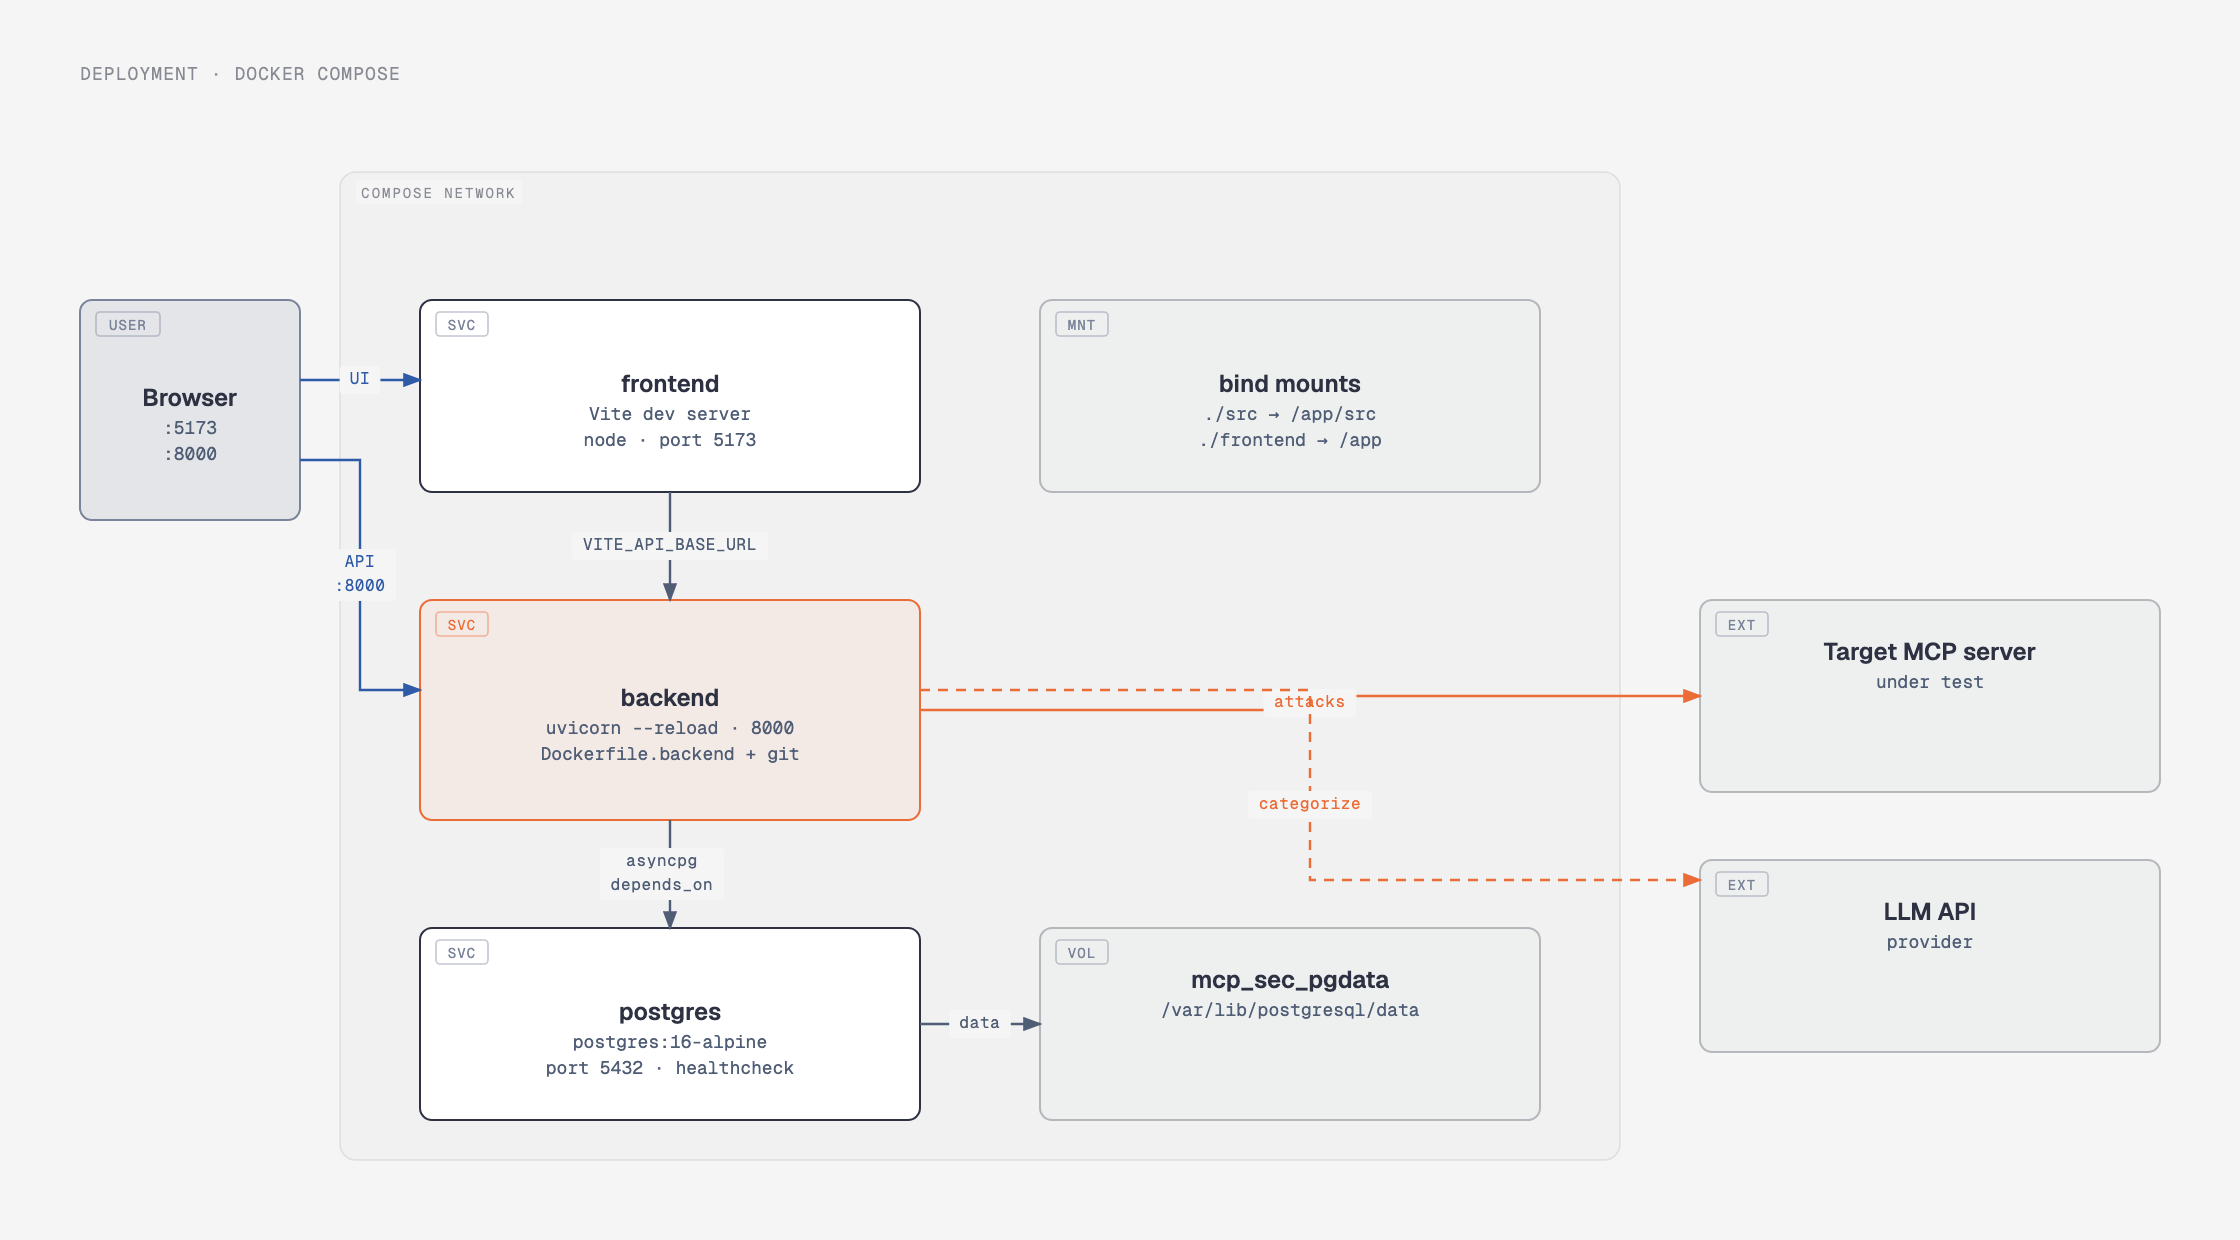
\includegraphics[width=\linewidth]{images/deploy-containers.png}
    \caption{Deployment: the three Docker Compose services, their host port
    mappings, the database volume, and the external target server and LLM API.}
    \label{fig:deploy}
\end{figure}

\section{The LLM Provider Abstraction and Observability}
\label{sec:llm-provider}

Every \gls{llm} call in the pipeline, attack synthesis and judging, passes through one method on a provider abstraction, \texttt{complete\_json}. Each provider implements that method, and each implementation is wrapped in a single tracing decorator. The payoff is twofold. A change to tracing is made once and applies to all three providers uniformly, including Ollama's raw HTTP path, which vendor-specific auto-instrumentation would have missed. And the one chokepoint is where model name and token usage are recorded, which is what later lets the cost of a scan be attributed per call.

The per-call records are grouped into one trace per scan. A scan opens a root span tagged with the target and the provider, and a child span per tool, so an entire scan reads as one tree, discover, categorize, then synthesize and judge for each tool, rather than a hundred disconnected calls. Tracing is a strict no-op when its keys are unset, and every traced call is wrapped so that a tracing fault can never break a scan. This keeps observability genuinely optional: a developer who sets no keys sees no behavioral change at all. Jev requests do not pass through the provider abstraction, since they use a different \gls{api}, but each one is recorded in the same trace with its request, response, and token usage.

\section{Classification with Jev and the Baseline Floor}
\label{sec:categorizer}

The classifier sends Jev each discovered tool's name, description, and input schema as the request state, together with one yes/no question per semantic category, eleven in all, grouped into requests of at most eight questions. Each question carries the category's description and instructs the model to treat the tool definition as untrusted data, to answer yes only when the category is the tool's primary attack surface, and not to infer hidden behavior. Jev returns a probability for each question. The classifier ranks the categories by probability, keeps those at or above a configurable threshold, 0.6 by default, and caps the result at a configurable number of categories per tool, currently one. These constraints keep the number of attacks a classification implies from inflating, and the threshold and cap can be tuned without changing the questions.

The floor described in Section~\ref{sec:decisions} is applied in code after the model answers. The generic fuzzing category is appended to every tool's result regardless of the probabilities, and if a Jev request fails, the tool receives the baseline categorization alone rather than being dropped. Neither a manipulated tool description nor a service failure can therefore remove a tool from the attack set. The earlier \gls{llm} classifier is kept in the codebase as a reference and serves as the baseline in the classification benchmark reported in Chapter~\ref{chap:results}.

\section{Payloads and Filter-Evasion Mutations}
\label{sec:payloads}

The payload library holds a fixed set of attack \glspl{payload} per category, and an adapter layer makes disclosed and synthetic payloads from the project's datasets available through the same interface. Fired as-is, one payload per category tests whether a vulnerable \gls{sink} responds, but it does not test whether a server's \emph{input filtering} can be walked around. A blocklist that rejects the literal string of a known injection may wave through an equivalent variant that an \gls{llm} still reads and obeys.

The mutation layer closes that gap. It models an \emph{operation} as a pure string-to-string transform, among them \texttt{base64}, \texttt{url\_encode}, \texttt{unicode\_escape}, \texttt{hex\_escape}, \texttt{homoglyph}, \texttt{zero\_width}, \texttt{whitespace\_pad}, and \texttt{rot13}, and a \emph{recipe} as an ordered chain of operations where each one's output feeds the next. Because the whole layer is pure transforms with no target, network, or model call, it is self-contained and trivially unit-tested. A mutated template keeps the original payload's success indicators, which is the point: a rule-based hit on an obfuscated variant means both that the obfuscation got past input filtering and that the underlying behavior still fired.

Two guards keep this honest. Latency- and count-based probes carry no textual success indicators, so they are skipped entirely; obfuscating a time-delay payload would break the very trigger its verdict depends on. And a recipe that does not change a given payload, such as a Unicode escape applied to pure ASCII, is not emitted, so the scan never fires a variant identical to its base. Mutations are applied by default only to the text-interpreted categories, where an encoded payload is still meaningful, and the feature is off unless explicitly enabled.

\section{Attack Synthesis and Execution}
\label{sec:executor}

A synthesized attack has to be a schema-valid call, or the server rejects it before the payload reaches any interesting code. The executor has two ways to produce one. The \gls{llm} path fills every required field other than the injection point with a plausible benign value, so the injected value actually reaches the tool's logic rather than producing a validation error that tests nothing. A static path fills placeholders directly; it is cheaper, works well for simple one- or two-field schemas, and is used automatically if the model call fails. The static path can also be forced globally for fully deterministic runs. Figure~\ref{fig:attack-sequence} shows the per-tool request and response sequence of the attack phase.

\begin{figure}[htbp]
    \centering
    % TODO: export images/impl-attack-sequence.svg to images/impl-attack-sequence.pdf
    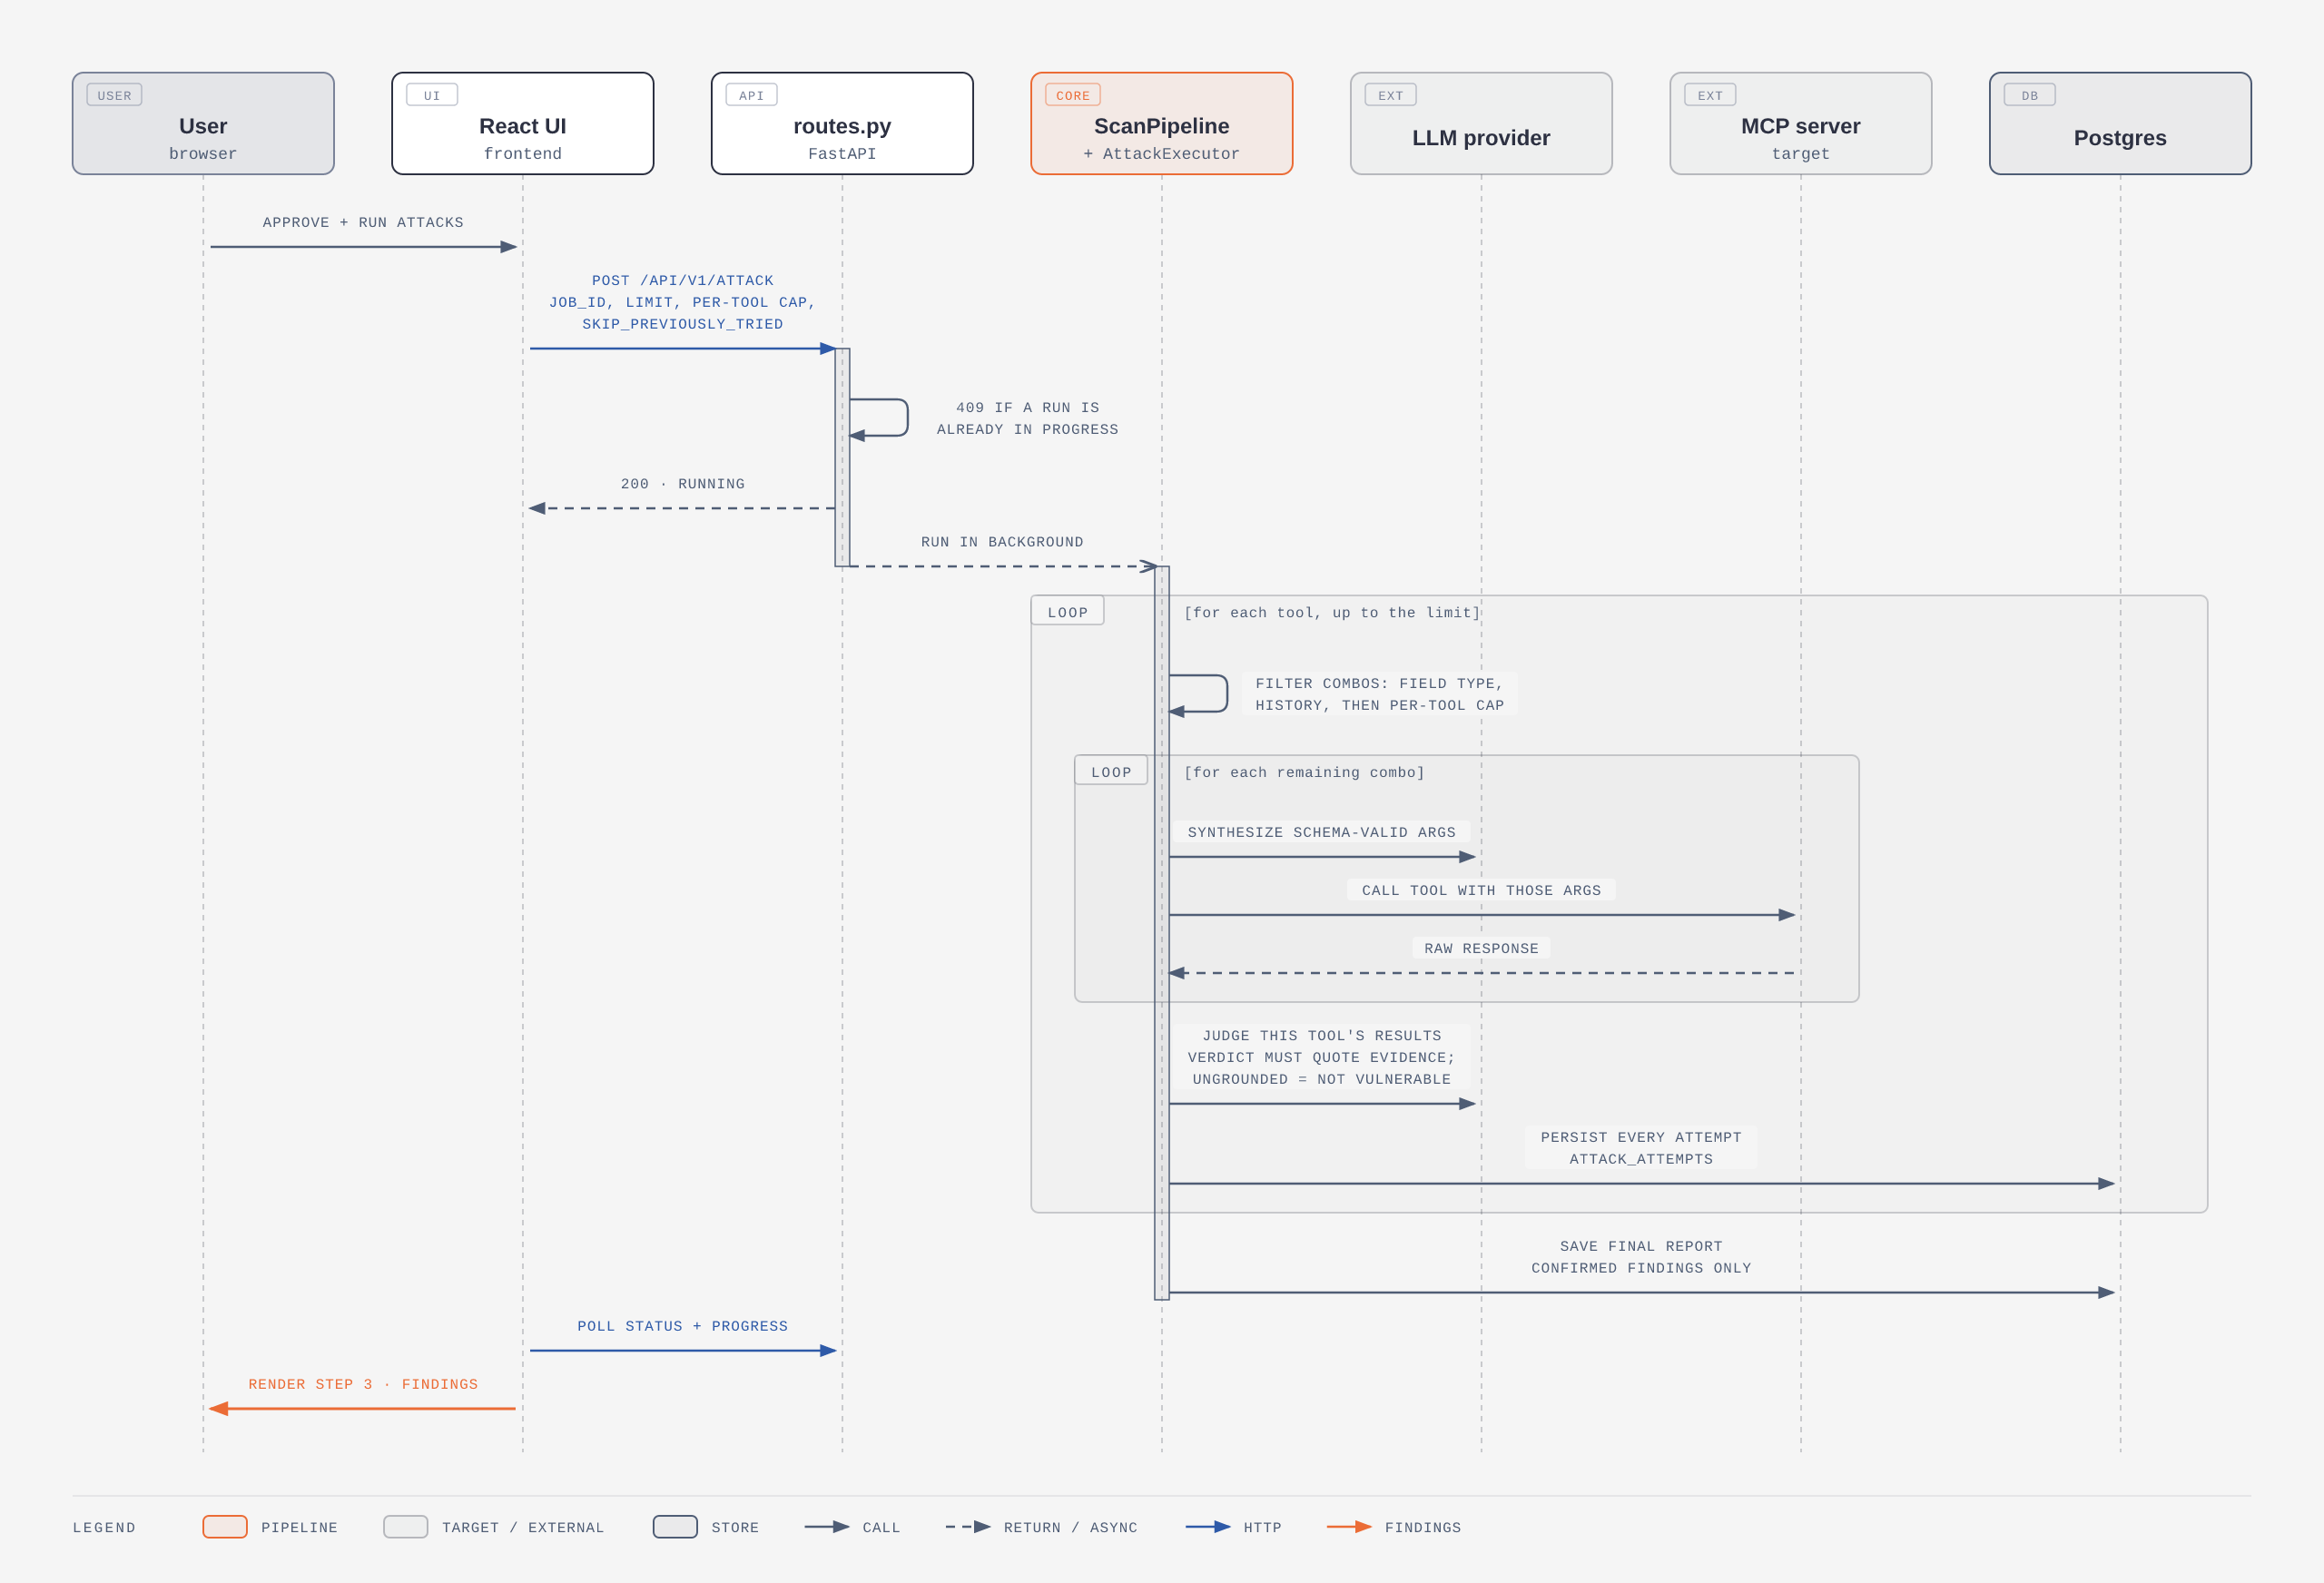
\includegraphics[width=\linewidth]{images/impl-attack-sequence.png}
    \caption{The attack phase: per-tool payload synthesis, live call, and judging.}
    \label{fig:attack-sequence}
\end{figure}

By default a run attacks one tool at a time, which keeps it deterministic and reproducible, the right baseline for measurement. Raising the concurrency cap attacks several tools at once in two phases: the non-timing payloads run concurrently, each tool in its own \gls{mcp} session because one shared session's concurrency safety is not guaranteed, and then the latency-based payloads run serially with nothing else in flight, so load cannot corrupt a timing verdict. The set of findings is the same either way; parallelism changes order and speed, not conclusions.

\section{Dual Evaluation and the Grounded Judge}
\label{sec:evaluator}

Evaluation runs the two checks introduced in Section~\ref{sec:decisions}. The rule-based check matches responses against known-format signatures and latency thresholds; it is fast, free, and precise, but it only sees what it was written to see. The \gls{llm} judge is invoked where semantics are needed, on confirmed rule-based hits for an explanation and a grounded evidence span, and on the categories that are inherently semantic, so the extra model call is spent only where it earns its place.

The judge is constrained rather than trusted. It must return the exact span of the response that proves the leak or the execution, and it is told, per category, that an error, refusal, validation failure, or timeout is a \emph{failed} attack unless the error itself is the disclosure, such as a traceback exposing internal paths or a database error revealing a schema. After the model answers, the code verifies that the quoted span is actually present in the response, normalized for whitespace and case and subject to a minimum length; if the quote is missing, empty, or too short, a ``vulnerable'' verdict is flipped to not-vulnerable, with the original reasoning kept for audit. Because this check is deterministic and model-agnostic, it catches a hallucinated success regardless of which provider or model produced it, while rule-based hits, already grounded in a concrete match, are left untouched.

\section{Authenticated Servers: the OAuth Flow}
\label{sec:oauth}

\gls{mcp} servers exposed over \gls{http} increasingly require \gls{oauth} rather than a static token~\cite{mcp2025spec}. The implementation builds entirely on the official \gls{sdk}'s OAuth client provider, so metadata discovery, \glsdisp{dynamic_client_registration}{dynamic client registration}, and \gls{pkce} are the SDK's responsibility, not reimplemented here. The protocol chain is the standard one~\cite{rfc6749}: the client asks the server which authorization server handles it, asks that server for its endpoints, obtains a client identifier, and completes an authorization-code grant with PKCE~\cite{rfc7636} as mandated for a public client that has no secret to keep confidential.

The flow is matched to a two-phase interface. A start call creates an in-memory connection and begins discovery in the background; its redirect handler opens the system browser to the authorize URL and records the OAuth state so the later callback can be matched to the right pending login. The provider blocks until the callback resolves it with the returned code, the SDK completes the token exchange internally, and discovery and classification then run over the now-authenticated session as the same step. The resulting bearer token is folded into the same process-local credential store every other transport uses, so the attack call needs no OAuth-specific code. Tokens and client information are reused per target \acrshort{url} for the life of the process and are never written to the database or to disk, consistent with the credential posture of Section~\ref{sec:data}.

Two interoperability issues encountered while building this are worth recording, because they are the kind of detail a practitioner repeating the work would hit. One provider, in the absence of an explicit token-endpoint authentication method at registration, defaulted new clients to a confidential-client method and issued a secret the tool had no business holding, after which the SDK sent the client identifier in two places at once and the authorization server rejected it; the fix was to request the public-client method explicitly at registration time. Another provider has no registration endpoint at all, returning a bare 404, which confirmed that dynamic registration is simply unimplemented there and motivated a manual escape hatch that pre-seeds the client information so the SDK skips registration entirely.

\section{Static Analysis Engine}
\label{sec:static-impl}

The static engine reads source and connects to nothing. Source arrives one of two ways, both refusing anything unsafe: a public repository is shallow-cloned over \gls{https} only, with other \acrshort{url} schemes refused and git never prompting for credentials, and then deleted after analysis; an uploaded folder is accepted only for the relevant file types, with absolute paths or paths containing parent-directory references rejected rather than sanitized. A safe file walk applies exclusions, file-count and size caps, and a refusal to follow symlinks out of the root. Figure~\ref{fig:static-flow} shows how a run moves from ingested source to attributed findings.

\begin{figure}[htbp]
    \centering
    % TODO: export images/impl-static-analysis.svg to images/impl-static-analysis.png
    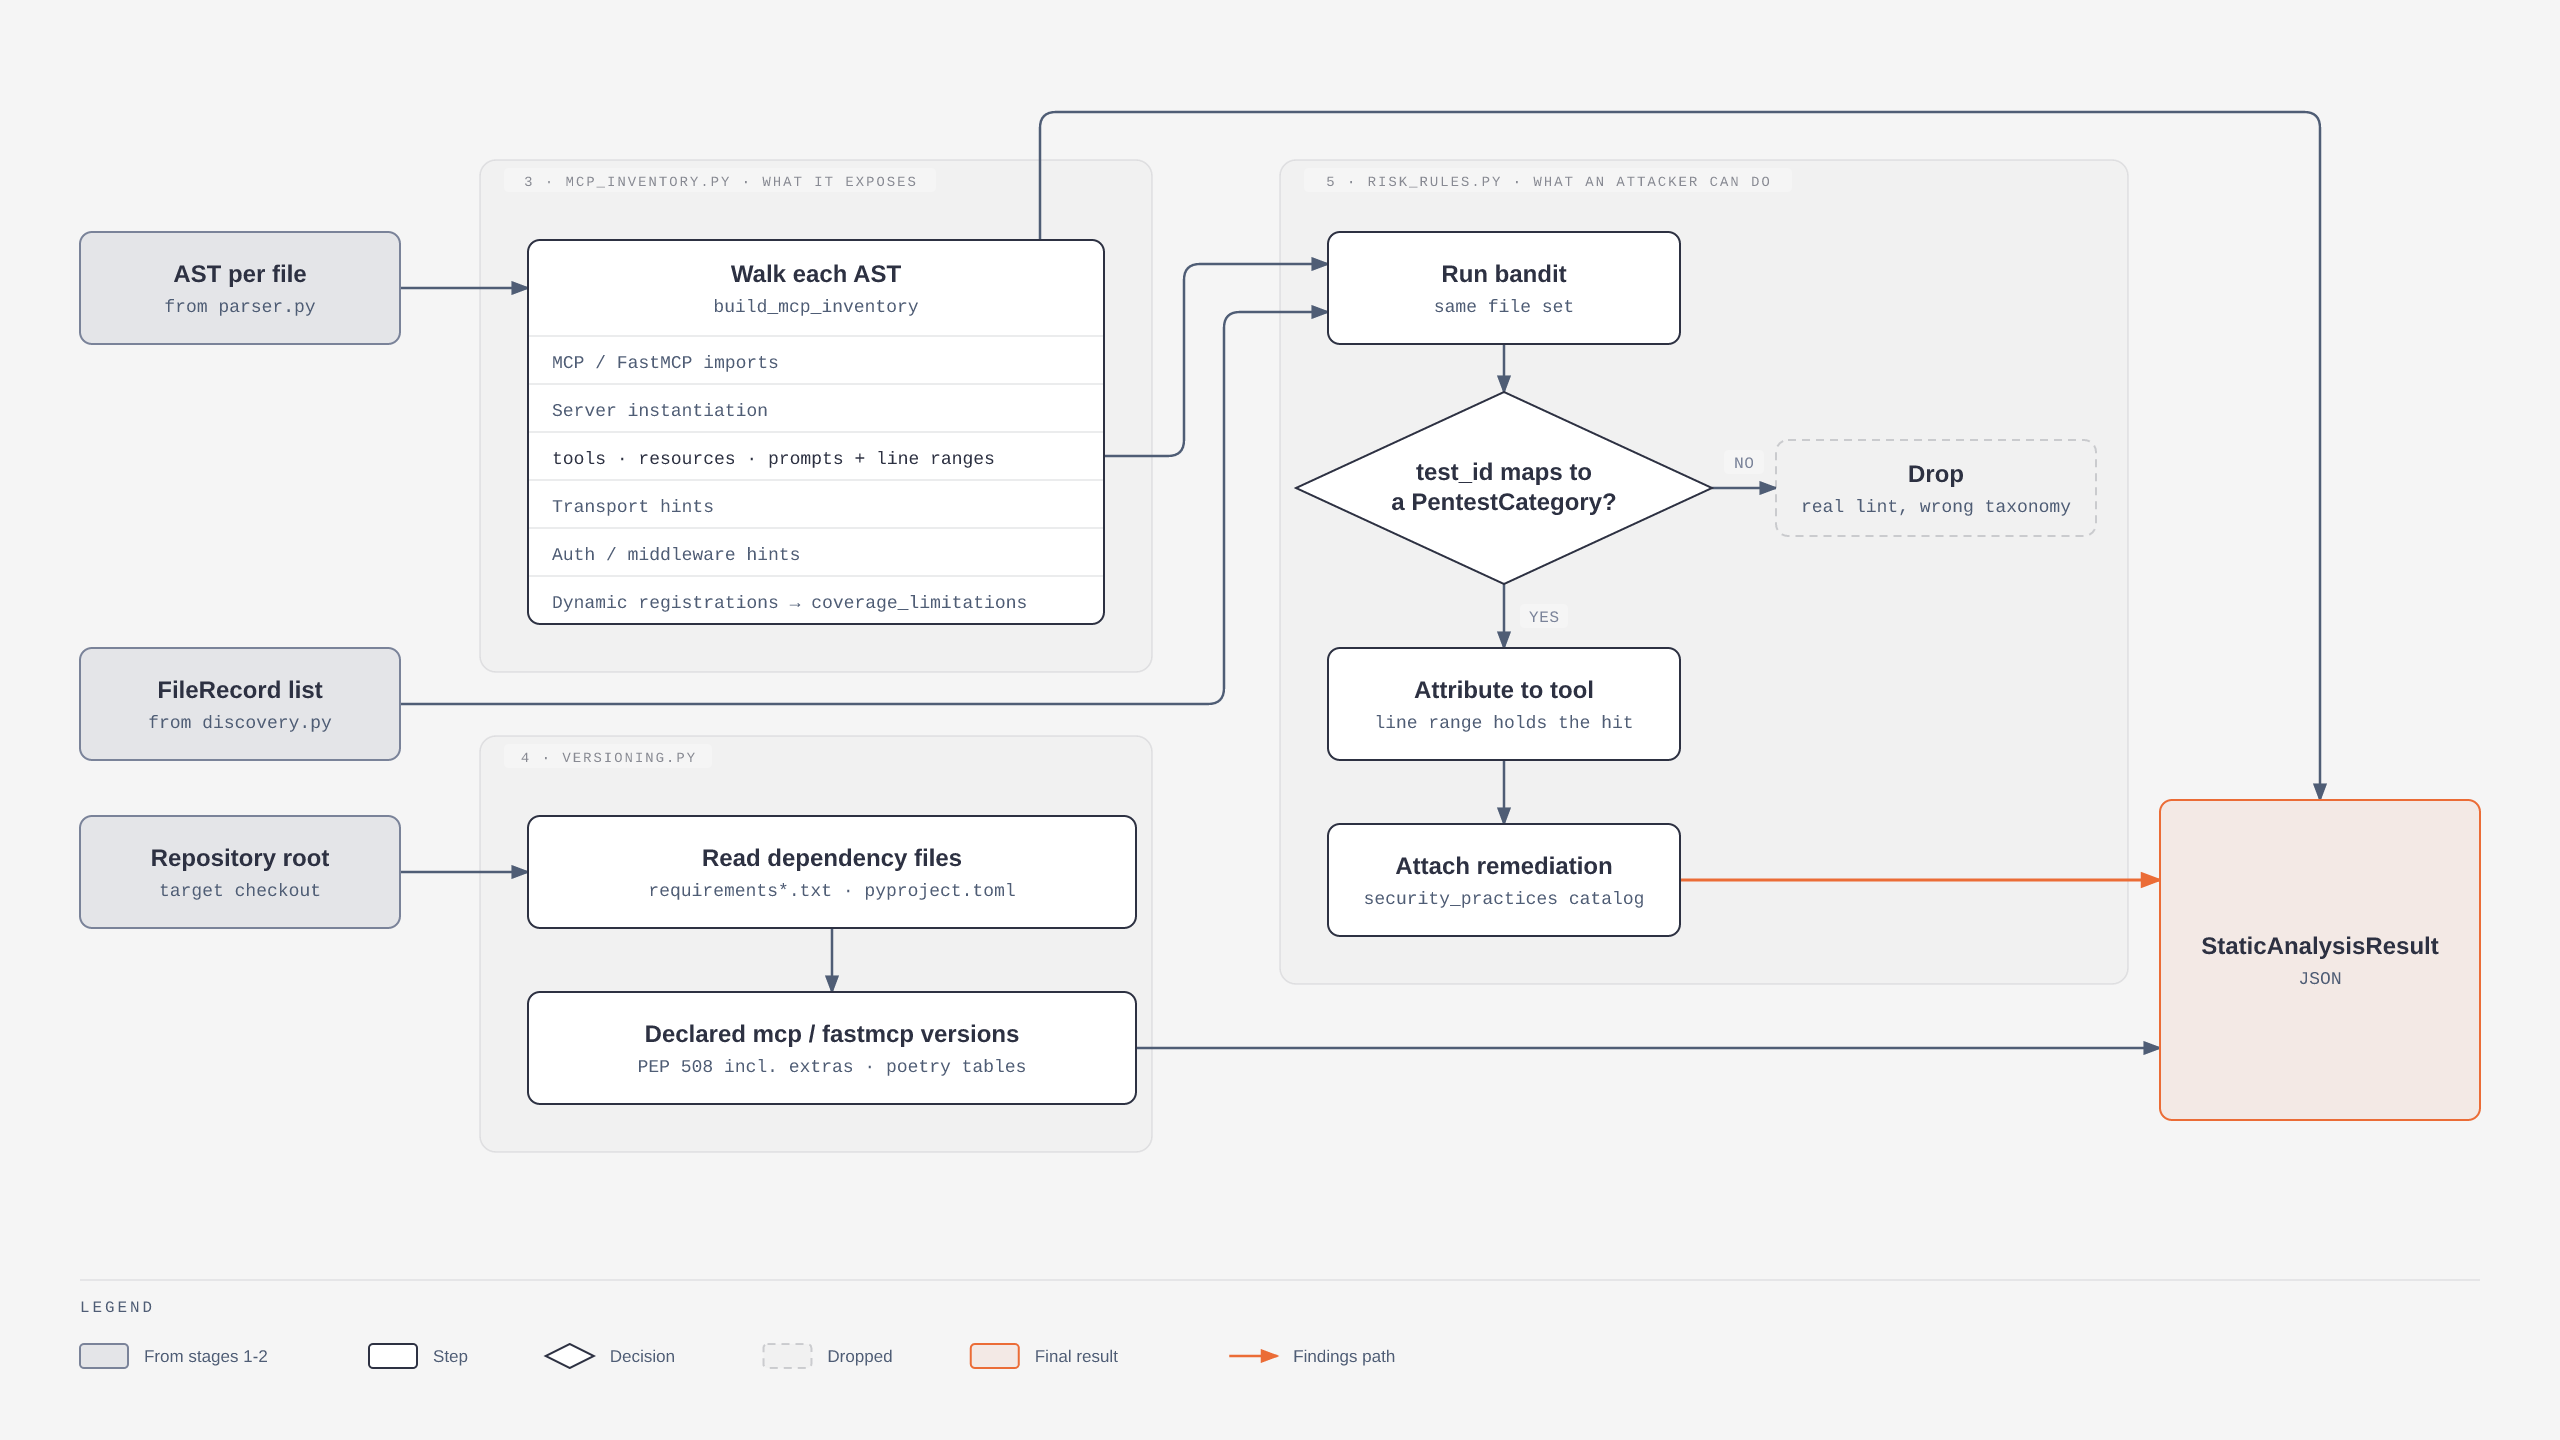
\includegraphics[width=\linewidth]{images/impl-static-analysis.png}
    \caption{Static analysis: parse, inventory the exposed surface, and attribute risk findings to the tool that exposes them.}
    \label{fig:static-flow}
\end{figure}

Each file is parsed to an \gls{ast}, and a syntax error is recorded while the run continues, so analysis is partial rather than all-or-nothing. The inventory pass is hand-written tree walking because it needs MCP-specific knowledge: which function is a registered tool, and where its body ends. It records the registrations with their parameters and line ranges, the transport, and authentication hints, and reads the declared MCP dependency version from the project's requirements. Risk detection reuses Bandit rather than hand-rolling sink matching; this engine's contribution is mapping Bandit's test identifiers onto the taxonomy and attributing each hit to the tool that exposes it. A shell-executing call maps to \gls{command_injection}, a string-built query to \acrshort{sql} injection, a pickle load to \glsdisp{deserialization_attack}{deserialization}, and a hit inside a registered tool's line range is attributed to that tool while a hit outside the taxonomy is dropped. The same analysis is available offline through a command-line entry point, so it can run with neither a server nor the web interface.

\section{Persistence Layer}
\label{sec:persistence}

The database is reached only through a repository component; it is the only code that touches the \gls{orm}, which keeps persistence concerns out of the rest of the pipeline and isolates any future schema change to one place. The \gls{json} columns are written to be portable across both SQLite and PostgreSQL, which is what lets the test suite run the full persistence layer against an in-memory SQLite database and still exercise the same code path production uses, including the round trip from a Pydantic model to a dictionary to database JSON and back that the attack orchestration depends on.

\section{Testing and Continuous Integration}
\label{sec:testing}

The test suite runs without network access. The Jev classifier has no unit tests yet; its behavior is measured instead by the classification benchmark in Chapter~\ref{chap:results}. The earlier \gls{llm} classifier is tested against a stubbed provider, covering the two floor-related failure modes. The persistence layer is tested against in-memory SQLite, including the JSON round trip. The static analysis tests cover both directions of its contribution: a dangerous call inside a registered tool must come back attributed to that tool, and a Bandit finding outside the taxonomy must be dropped rather than reported. A parity test keeps the frontend's copy of the taxonomy in sync with the Python enumerations, and the remediation catalog is checked so that every category resolves to remediation text. 
The same parity check requires every category to carry a valid \gls{cvss} vector, and a deterministic test fixes one known vector, the \gls{sql} injection one, to its expected score of 9.4, its Critical band, and its high, high, low impact, so a change in the library or the catalog cannot silently shift the scores reported in Chapter~\ref{chap:results}.
Continuous integration runs the suite together with Bandit, \texttt{pip-audit}, and \texttt{detect-secrets} on every push, and the latter three currently pass clean against the codebase, verified in CI rather than assumed.

\chapter{Results and Discussion}
\label{chap:results}

% =====================================================================
% OUTLINE CHAPTER. Framework and ground truth are real; every number is a
% placeholder to be filled from actual scan runs. Do not invent figures.
% Fill order: run each victim server (targets/), run discover+attack, record
% per-category outcome, then fill Tables 5.x and the benchmark numbers.
% =====================================================================

This chapter evaluates the tool. It describes the evaluation design and the corpus of targets, reports the benchmark and detection results, compares the static and dynamic paths on the same servers, and discusses what the results do and do not establish, including the threats to their validity.

\section{Evaluation Design}
\label{sec:eval-design}

% WRITE-UP NOTES:
% - Restate the research question (Section 1.2) as the thing being measured.
% - Metrics (named in the method, Chapter 1): vulnerability detection rate,
%   false-positive rate, attack coverage, performance overhead.
% - Ground truth: the 9 victim servers in targets/. Each pairs a genuinely
%   exploitable tool with a SAFE CONTROL of the same shape. This is the label:
%   a correct scan flags the vulnerable tool and leaves the control alone.
%   => detection rate from the vulnerable tools, false-positive rate from the
%      controls. State this is a small, author-built corpus (threat to validity).
% - Secondary corpus: datasets/ (88 entries: 27 documented real-world
%   incidents/CVEs + 61 synthetic payloads), used as the payload source and as
%   external grounding for the taxonomy, not as a detection benchmark.
% - Environment: sequential baseline (MAX_CONCURRENT_TOOLS=1), which model /
%   provider, which mutation setting. Record for reproducibility.

The evaluation is built around the nine intentionally-vulnerable MCP servers that ship with the project. Each server is a single file that pairs a genuinely exploitable tool with a safe control tool of the same shape, so a correct scan flags the first and leaves the second untouched. That pairing is the ground truth: the exploitable tools yield the detection rate, and the controls yield the false-positive rate. Table~\ref{tab:targets} lists the corpus.

\begin{table}[htbp]
\centering
\small
\begin{tabular}{p{3.0cm} p{4.2cm} p{3.0cm} p{2.6cm}}
\hline
\textbf{Server} & \textbf{Category} & \textbf{Vulnerable tool} & \textbf{Safe control} \\
\hline
db & sql\_injection & run\_query & find\_user \\
devops & command\_injection, dos & ping\_host, grep\_logs & run\_command\_safe \\
files & path\_traversal & read\_file & read\_doc \\
fetch & ssrf & fetch\_url & fetch\_allowlisted \\
secrets & information\_extraction & get\_config & get\_public\_config \\
notes & resource\_extraction, memory poisoning & list\_all\_notes, save\_note & get\_my\_notes \\
admin & auth\_access\_control & promote\_user & whoami \\
parser & deserialization & load\_config & load\_json \\
assistant & jailbreak / prompt injection & summarize & safe\_summarize \\
\hline
\end{tabular}
\caption{The victim-server corpus. Each vulnerable tool has a matched safe control.}
\label{tab:targets}
\end{table}

% Note honestly here: two categories are known-under-detected by the current
% executor (auth_access_control needs a low-priv session; cross-session memory
% poisoning needs a second session). These are expected misses, documented, and
% belong in the discussion, not hidden.

\section{Benchmarks}
\label{sec:benchmarks}

% WRITE-UP NOTES — fill from real runs:
% - Per-server: #tools discovered, #categories assigned, #attacks sent,
%   wall-clock scan time, LLM token usage / estimated cost (from Langfuse).
% - Report the sequential baseline; if parallelism was measured, report the
%   speedup and confirm the finding SET was identical (only order/speed changed).
% - Mutation on vs off: effect on #attacks sent and on detections.

\begin{table}[htbp]
\centering
\small
\begin{tabular}{p{2.6cm} r r r r r}
\hline
\textbf{Server} & \textbf{Tools} & \textbf{Categories} & \textbf{Attacks} & \textbf{Time (s)} & \textbf{Cost} \\
\hline
db & TODO & TODO & TODO & TODO & TODO \\
devops & TODO & TODO & TODO & TODO & TODO \\
\dots & & & & & \\
\hline
\end{tabular}
\caption{Per-scan benchmarks on the victim corpus (sequential baseline). TODO: fill from runs.}
\label{tab:benchmarks}
\end{table}

\section{Detection Results}
\label{sec:detection}

% WRITE-UP NOTES — fill from real runs:
% - One row per server. Columns: vulnerable tool flagged? (expected yes),
%   control flagged? (expected no), confidence, evidence span quoted by judge.
% - Compute detection rate = flagged vulnerable / total vulnerable;
%   false-positive rate = flagged controls / total controls.
% - Call out the grounded-judge overrule count: how many "vulnerable" verdicts
%   were flipped because the evidence quote was absent. This is a key result:
%   it is the false-positive-suppression mechanism doing visible work.
% - Add a column "Max CVSS" per server (ScanReport.max_cvss) to the
%   per-server table; it is the single aggregate metric of a scan.
% - Severity counts per band come from CVSS, so they are comparable across
%   providers/models (the judge no longer sets severity).

\begin{table}[htbp]
\centering
\small
\begin{tabular}{p{2.6cm} p{2.4cm} p{2.4cm} p{2.0cm} p{2.4cm}}
\hline
\textbf{Server} & \textbf{Vuln. flagged} & \textbf{Control flagged} & \textbf{Conf.} & \textbf{Evidence} \\
\hline
db & TODO & TODO & TODO & TODO \\
\dots & & & & \\
\hline
\end{tabular}
\caption{Detection outcome per server. Expected: vulnerable flagged, control not. TODO: fill from runs.}
\label{tab:detection}
\end{table}

\section{Static versus Dynamic Agreement}
\label{sec:agreement}

% WRITE-UP NOTES:
% - Run the static analyzer over the same 9 server source files and compare,
%   per category, against the dynamic findings.
% - Three buckets: (a) both agree, (b) static flagged code the live payload
%   could not reach, (c) a live finding with no static signal.
% - This comparison is itself a result: the shared taxonomy makes it a join.

\section{Discussion}
\label{sec:discussion}

% WRITE-UP NOTES — interpret, don't just restate the tables:
% - What the detection/false-positive numbers say about the research question.
% - The two known misses (auth, cross-session poisoning): honest gaps, with the
%   executor limitation that causes each, not server bugs.
% - Effect of the grounded judge on false positives (from the overrule count).
% - Effect of mutations on filter-bypass categories.
% - Threats to validity: small author-built corpus; confidence is the model's
%   self-report, not calibrated; timing-based checks are noisy under load.
%   These set up the limitations and future work in Chapter 6.
% - Note that every finding of one category gets the same score; the score
%   ranks classes of weakness, not the specific evidence of a finding.
\chapter{Conclusion}
\label{chap:conclusion}

% =====================================================================
% OUTLINE CHAPTER. Bullet notes mark what each section argues. Write as prose
% once Chapter 5 numbers exist, so contributions and limitations cite results.
% =====================================================================

% WRITE-UP NOTES: open by answering the research question from Section 1.2
% directly, in one or two sentences, grounded in the Chapter 5 results. Avoid a
% hollow recap; say what was shown, then move to contributions.

\section{Contributions}
\label{sec:contributions}

% The defensible novelty claims (what existing tools do NOT already do):
% - Automated LLM classification of unknown tools against a fixed taxonomy,
%   rather than a human deciding per tool, or a fixed rule set run at everything.
% - LLM-assisted payload synthesis that adapts to arbitrary tool schemas,
%   instead of hand-written test cases per tool shape.
% - Dual rule-based + grounded LLM-judge evaluation: catches known-format and
%   semantic leaks, and overrules an un-evidenced "vulnerable" verdict.
% - A deliberate, documented answer to "does the triage step itself trust
%   untrusted tool descriptions?" (the categorizer floor) — the tool's own
%   LLM step is exposed to the injection it detects, and the design addresses it.
% - One taxonomy and one remediation catalog spanning a dynamic and a static
%   path, so a static finding and a live finding are directly comparable.

\section{Limitations}
\label{sec:limitations}

% From the project's own "known limitations" — state them plainly:
% - Confidence scores are the model's self-report, not a calibrated metric; no
%   precision/recall against a large labeled corpus yet (the victim corpus is
%   small and author-built).
% - Timing-based checks (blind SQLi, DoS) are noisy under load / slow networks.
% - The static payload library is illustrative (DAST-level), not exhaustive.
% - In-memory credential store does not survive a restart or multiple workers.
% - No auth on the API itself (matches the "local application" scope).
% - resource_extraction wildcard probe has no automated success indicator.
% - Cross-session tests (memory poisoning, cross-tenant) are single-session in
%   the current executor; auth test lacks a low-privilege session.
% - No OAuth token auto-refresh between discover and attack; OAuth assumes the
%   backend and browser share a machine.
% - Static attribution is co-location (sink inside a tool's body), not data-flow
%   proof that a parameter reaches the sink; non-Python servers are unparsed.

\section{Future Work}
\label{sec:future}

% Roughly priority-ordered for the research:
% - Build and run a precision/recall benchmark against a larger labeled corpus
%   of vulnerable and known-safe servers — turns "seems to work" into a number.
% - Automate the two-session tests so the auth and cross-session categories are
%   actually exercised (removes the two known misses in Chapter 5).
% - Correlate the static and dynamic paths on one target and report where they
%   agree, where static reached what the payload could not, and vice versa.
% - Static analysis: data-flow instead of co-location; parse non-Python
%   (TypeScript) servers.
% - Normalize findings into their own indexed table; add schema migrations.
% - Add authentication to the API if it ever runs beyond the local machine.
% - Expand payload coverage per category (encoding variants, blind techniques).

\section{Final Remarks}
\label{sec:final}

% WRITE-UP NOTES: one short, substantive paragraph. State what the artifact
% establishes about securing MCP servers and why the taxonomy-shared, two-path
% design is the reusable idea beyond this specific tool. No generic summary.


% Limitations:
% - Scores are category-level base scores: an SQL error message and a full
%   table dump both get 9.4. Temporal and environmental CVSS metrics are not
%   used, so the score ignores exploit maturity and the deployment context.
% Future work:
% - Let the grounded judge adjust the C/I/A metrics per finding from the
%   evidence (e.g. raise C when real data leaked), keeping the rest of the
%   base vector, and recompute the score.
% - Evaluate CVSS v4.0 once tooling support is mature.

\bibliography{biblio}

\end{document}
